\documentclass[11pt,a4paper]{article}

\usepackage[a4paper,margin=1in]{geometry}
\IfFileExists{newtxtext.sty}{\usepackage{newtxtext,newtxmath}}{\usepackage{mathptmx}}
\usepackage[T1]{fontenc}
\usepackage[utf8]{inputenc}
\usepackage{microtype}
\usepackage{setspace}
\linespread{1.18}
\usepackage{booktabs}
\usepackage{array}
\usepackage{multirow}
\IfFileExists{threeparttable.sty}{\usepackage{threeparttable}}{%
  \newenvironment{threeparttable}{}{}%
  \newenvironment{tablenotes}{\par\vspace{2pt}\footnotesize\renewcommand{\item}{\par\noindent}}{\par}%
}
\usepackage{graphicx}
\usepackage{caption}
\captionsetup{labelfont=bf,font=small,skip=4pt}
\IfFileExists{placeins.sty}{\usepackage{placeins}}{\providecommand{\FloatBarrier}{\clearpage}}
\usepackage{tikz}
\usetikzlibrary{arrows.meta,positioning,shapes.geometric,fit,calc}
\usepackage[round,authoryear]{natbib}
\IfFileExists{apalike2.bst}{\bibliographystyle{apalike2}}{\bibliographystyle{plainnat}}
\usepackage[colorlinks=true,citecolor={blue!60!black},linkcolor={blue!60!black},urlcolor={blue!60!black}]{hyperref}

\graphicspath{{../wpi/outputs/figures/}{../improved-v2/outputs/figures/}}

\setlength{\parskip}{2pt}
\setlength{\parindent}{1.2em}

\title{\bfseries From crude oil to consumer inflation:\\ transmission and attenuation across India's price system}
\author{Aniket Pandey}
\date{April 2026}

\begin{document}
\maketitle

\begin{abstract}
\noindent India imports more than four fifths of the crude it consumes, yet the way that imported cost shock travels through domestic prices is uneven. This paper studies oil pass-through as a layered process. We trace it across four price tiers: wholesale headline inflation, retail petrol pricing at the pump, fuel-sensitive wholesale and consumer indices, and the headline consumer price index. The empirical core uses short-run asymmetric autoregressive distributed lag models with Newey--West inference, estimated on monthly series chained back to 1983 for headline WPI and to 1995 for the fuel and power component. A complementary nonlinear ARDL battery in levels is reported in the appendix. Three patterns hold up consistently. Pass-through into headline WPI is statistically detectable but small (cumulative pass-through of about 0.030 for positive oil shocks); it is roughly an order of magnitude larger in retail petrol and in fuel-sensitive wholesale prices; and it weakens sharply by the time the shock reaches headline CPI, where the cumulative effect is not significantly different from zero. A pre/post-2010 split shows that headline pass-through is materially larger in the post-deregulation regime, broadly consistent with the institutional shift toward market-linked pricing of transport fuels. Short-run asymmetry is not a robust feature of the preferred specifications. We read these results as evidence that imported oil inflation in India is best understood as a transmission-and-attenuation chain in which the pricing institutions and the basket composition of the consumer index together absorb most of the upstream shock before it reaches household inflation.
\end{abstract}

\noindent\textbf{Keywords:} oil price pass-through; imported inflation; India; wholesale inflation; consumer inflation; retail fuel pricing; deregulation; asymmetry.

\bigskip

\section{Introduction}
\label{sec:intro}

India is a structural net importer of crude oil. The country sourced close to 87 percent of its crude requirement from abroad in 2023--24, which makes the rupee value of a barrel of Brent one of the most directly observable cost shocks the domestic price system absorbs in any given month \citep{ppac2024}. The macro question that follows is old and policy-relevant: when crude moves, how much of that move ends up in the inflation rate that households actually face?

Existing work on India tends to answer that question one index at a time. Some studies look at WPI in isolation \citep{bhoi2012,suresh2026}. Some look at CPI subgroups or aggregate CPI \citep{abubakar2018,sek2019}. Others zoom in on the retail fuel pricing channel after the 2010 petrol deregulation and the October 2014 diesel deregulation \citep{pradeep2022,deheri2024}. Each of these strands says something useful. Read together, they also leave a gap: India's pricing institutions sit in a chain (international crude $\to$ exchange rate $\to$ domestic refined products $\to$ wholesale energy $\to$ consumer fuel $\to$ headline CPI), and the academic literature rarely walks the chain end-to-end on a single sample. The result is that two true statements coexist uneasily in the policy discourse. Oil shocks pass through significantly to wholesale inflation. Oil shocks barely move headline CPI. Both can hold at the same time. The question is where in the chain the shock actually dissipates.

This paper takes that chain seriously and estimates pass-through at four points along it. The headline WPI series is built by chaining four official base years (1981--82, 1993--94, 2004--05, 2011--12) into a single 528-observation monthly series running April 1982 through March 2026, which gives the longest historically defensible wholesale inflation horizon currently available for India. The WPI Fuel and Power subindex is chained over three base years and runs April 1994 through March 2026. The retail fuel layer is the PPAC monthly Delhi retail selling price for petrol from August 2004 onward. Headline CPI on the All-India 2010=100 base is the consumer endpoint. To these we add the CPI Fuel and Light subgroup as a short bridge series. Because of the post-2011 CPI rebase, the fuel-and-light series is treated as a supporting layer and not as one of the headline mandates.

The empirical strategy is deliberately unfussy. The main models are short-run asymmetric ADL specifications in log-differences. Each model has twelve own lags, lags zero to six on positive and negative oil-change components, month fixed effects, and Newey--West HAC standard errors. Cumulative pass-through is reported as the sum of the positive (CPT$^+$) and negative (CPT$^-$) coefficients, with Wald tests on each sum and on the symmetry restriction CPT$^+$ = CPT$^-$. A bootstrap symmetry test using a restricted-residual circular block scheme provides finite-sample inference. A nonlinear ARDL battery in levels, with bounds testing in the manner of \citet{pesaran2001} and the asymmetric decomposition of \citet{shin2014}, is reported in the appendix as supplementary long-run evidence.

The headline numbers tell a layered story. In the long historical sample, wholesale inflation responds to rupee oil shocks with CPT$^+ = 0.030$ ($p = 0.024$) and CPT$^- = 0.037$ ($p = 0.001$). The point estimates are small but precise, and asymmetry is not rejected (asymptotic $p = 0.673$, bootstrap $p = 0.746$). Pre/post-2010 splits show that essentially all of this signal sits in the post-deregulation period, where CPT$^+$ rises to $0.074$ and CPT$^-$ to $0.081$. Move down to the fuel-sensitive layer and the magnitudes change qualitatively. WPI Fuel and Power has CPT$^+ = 0.287$ and CPT$^- = 0.268$, both with $p < 0.001$. PPAC retail petrol responds even more strongly, with CPT$^+ = 0.346$ and CPT$^- = 0.191$ on a 245-month sample beginning in August 2004. By the time the shock reaches headline CPI, the picture is almost the opposite of the wholesale fuel result. CPT$^+ = 0.021$ with $p = 0.122$ and CPT$^- $ is essentially zero ($p = 0.94$). Most of the upstream movement has been absorbed somewhere between the pump and the consumer basket.

Three contributions follow. First, we provide a single-paper map of where the oil signal travels and where it disappears, rather than treating WPI and CPI as competing answers to the same question. Second, the long historical wholesale sample lets us anchor the central pass-through estimate in a 43-year window, which is unusual for the India literature; most existing wholesale studies stop in the 2010s. Third, the integrated design forces a reframing of the asymmetry debate. Short-run asymmetry is not the most robust feature of the data. Attenuation across layers is. The novelty here is in integration and not in estimator innovation, and we take care not to oversell it.

The rest of the paper is organised as follows. Section \ref{sec:back} sketches the institutional backdrop and positions the analysis against the existing literature. Section \ref{sec:data} describes the data and the empirical strategy. Section \ref{sec:wpi} reports the historical wholesale results. Section \ref{sec:mech} traces the mechanism and the attenuation across the four layers, which is the paper's signature section. Section \ref{sec:rob} reports robustness exercises and summarises the appendix NARDL evidence. Section \ref{sec:conc} draws the policy implications.

\section{Institutional background and focused literature}
\label{sec:back}

Two institutional facts shape the way oil shocks enter Indian inflation. The first is the foreign exchange channel. Brent is denominated in dollars and India settles oil imports in dollars, so the rupee cost of a barrel is the product of Brent and the INR/USD exchange rate. A textbook rupee depreciation of five percent against a flat Brent price feeds into the same imported cost as a five percent Brent rise against a flat exchange rate. The second is the domestic pricing regime for refined products, which has changed substantially over the sample. From the 1970s through the early 2000s, India operated an Administered Pricing Mechanism in which the union government set retail prices for petrol, diesel, kerosene and LPG and absorbed the gap between domestic and import-parity prices through subsidies and oil bonds. The mechanism was wound down in steps. Petrol was deregulated in June 2010. Diesel followed in October 2014. Kerosene and LPG have remained partially subsidised. Tax components (central excise plus state VAT) have grown into a large share of the pump price, which gives the union government a non-trivial buffer against international price movements.

These two facts together generate an empirical prediction. In a fully market-linked retail fuel regime, an oil shock should travel quickly to retail petrol and diesel. From there it should move into the fuel-sensitive subcomponents of the wholesale and consumer indices. Whether it reaches headline inflation depends on the weight of fuel-sensitive items in the index and on whether non-fuel components move in the same direction. In an administered regime, the same shock should be largely absorbed at the retail stage by changes in subsidy bills and excise schedules. The pre- and post-2010 subsamples thus offer a natural test of whether deregulation made the pass-through chain more permissive.

The Indian literature on oil pass-through can be read as a sequence of partial answers to this combined institutional setup. Early work using linear vector autoregressions and cointegration tests on WPI typically reported small but significant pass-through coefficients \citep{bhoi2012,bhanumurthy2012}. A second wave moved to nonlinear ARDL methods to test for asymmetry. \citet{abubakar2018} report long-run asymmetric pass-through to Indian inflation using NARDL. \citet{chattopadhyay2015} and \citet{pal2016} examine asymmetry in oil product prices and find that asymmetric behaviour is concentrated in the segments where market-linked pricing actually applies. \citet{pandey2019} document partial pass-through of crude to retail fuel in the early post-deregulation window. \citet{pradeep2022} focuses on the diesel reform and reports that asymmetric pass-through to disaggregated wholesale and consumer prices is sharper in the post-reform window. \citet{deheri2024} document asymmetric pass-through from crude to retail fuel. Two more recent contributions inform the present design. \citet{suresh2026} estimate a NARDL system on Indian wholesale prices and report long-run asymmetry with weaker short-run asymmetry, which is broadly consistent with what the appendix evidence here will show. \citet{sek2019} provides cross-country panel evidence that the WPI--CPI gap in pass-through is wider in oil importers, which is a useful comparative anchor.

What none of these studies do is build a single empirical architecture that runs the full chain from crude to headline CPI on consistent monthly data. Most pick one estimator family (NARDL or SVAR or VECM) and one inflation index, and report a pass-through estimate together with a sign of asymmetry. The headline-versus-fuel-sensitive contrast is sometimes noted in passing, but the attenuation across layers is rarely the object of inference. \citet{sadath2021}, using an SVAR, gets closest to this layered framing for the macro-level response, although the focus there is on real activity rather than on pricing institutions. The contribution of the present paper is more architectural than methodological. We retain the now-standard short-run asymmetric ADL as the workhorse, push NARDL to the appendix, and use the gap between the four pass-through estimates as the substantive object of study.

A short methodological note is in order. The Indian pass-through literature has occasionally treated headline WPI as a stand-in for input-cost inflation and headline CPI as a stand-in for household-facing inflation, then disagreed about which is the right object of policy. We sidestep that debate. WPI and CPI answer different questions. WPI is informative about upstream cost transmission and imported input pressures. CPI is informative about household-facing inflation. Studying both jointly lets the paper distinguish where oil shocks enter the price system from whether they survive all the way to consumer inflation. The post-2014 monetary policy framework that targets headline CPI \citep{rbi2014} makes the CPI endpoint the right place to evaluate household impact, but it does not make wholesale evidence irrelevant. If anything, the wholesale evidence becomes more interesting once we know it is not mechanically reflected in the target.

\section{Data and empirical strategy}
\label{sec:data}

The dataset is monthly. Brent crude in US dollars per barrel comes from the World Bank Commodity Markets Pink Sheet. The INR/USD spot rate comes from FRED (series \texttt{EXINUS}). The rupee oil price is constructed as the product of Brent and EXR. Wholesale prices come from the Office of the Economic Adviser (OEA) under the Department for Promotion of Industry and Internal Trade. Headline WPI and the WPI Fuel and Power subindex are constructed by chain-linking the four official OEA base series (1981--82, 1993--94, 2004--05 and 2011--12) using the official linking factors, with all series rebased to 2011--12 = 100. This gives a 528-observation headline series running April 1982 through March 2026 and a 384-observation Fuel and Power series running April 1994 through March 2026. The retail fuel layer is the PPAC monthly Delhi retail selling price for petrol, available from August 2004. The consumer endpoint is the All-India headline CPI series. The CPI Fuel and Light subgroup is taken from the post-2011 base and used as a supporting bridge series rather than as a primary index. After inner joins on common dates, the active estimation samples cover roughly 43 years for headline WPI, 31 years for WPI Fuel and Power, and 20 years for the PPAC and CPI specifications. Table \ref{tab:data} summarises the series.

\begin{table}[t]
\centering
\caption{Series, sources, transformations, and sample spans.}
\label{tab:data}
\footnotesize
\setlength{\tabcolsep}{4pt}
\begin{threeparttable}
\begin{tabular}{p{3.4cm} p{4.4cm} p{1.6cm} p{3.0cm}}
\toprule
Series & Source & Transform. & Active sample \\
\midrule
Brent crude (USD/bbl) & World Bank Pink Sheet & $\Delta \ln$ & 1983-05 to 2026-03 \\
INR/USD spot rate & FRED \texttt{EXINUS} & $\Delta \ln$ & 1983-05 to 2026-03 \\
Rupee oil price & Brent $\times$ EXR (constructed) & $\Delta \ln$ & 1983-05 to 2026-03 \\
Headline WPI (2011-12 = 100) & OEA, chained across four bases & $\Delta \ln$ & 1983-05 to 2026-03 \\
WPI Fuel \& Power (2011-12 = 100) & OEA, chained across three bases & $\Delta \ln$ & 1995-05 to 2026-03 \\
PPAC retail petrol, Delhi & Petroleum Planning and Analysis Cell & $\Delta \ln$ & 2004-08 to 2024-12 \\
Headline CPI (All-India, 2010 = 100) & MoSPI / FRED \texttt{INDCPIALLMINMEI} & $\Delta \ln$ & 2004-08 to 2024-12 \\
CPI Fuel \& Light (post-2011 base) & MoSPI & $\Delta \ln$ & 2011-05 to 2024-12 \\
\bottomrule
\end{tabular}
\begin{tablenotes}\footnotesize
\item Notes: Wholesale series chained to a common 2011--12 = 100 base using OEA linking factors. Active samples reported after inner joins on common dates. The CPI Fuel \& Light series begins in May 2011 because the post-2011 base is the longest harmonised consumer fuel index currently available.
\end{tablenotes}
\end{threeparttable}
\end{table}


\begin{figure}[t]
\centering
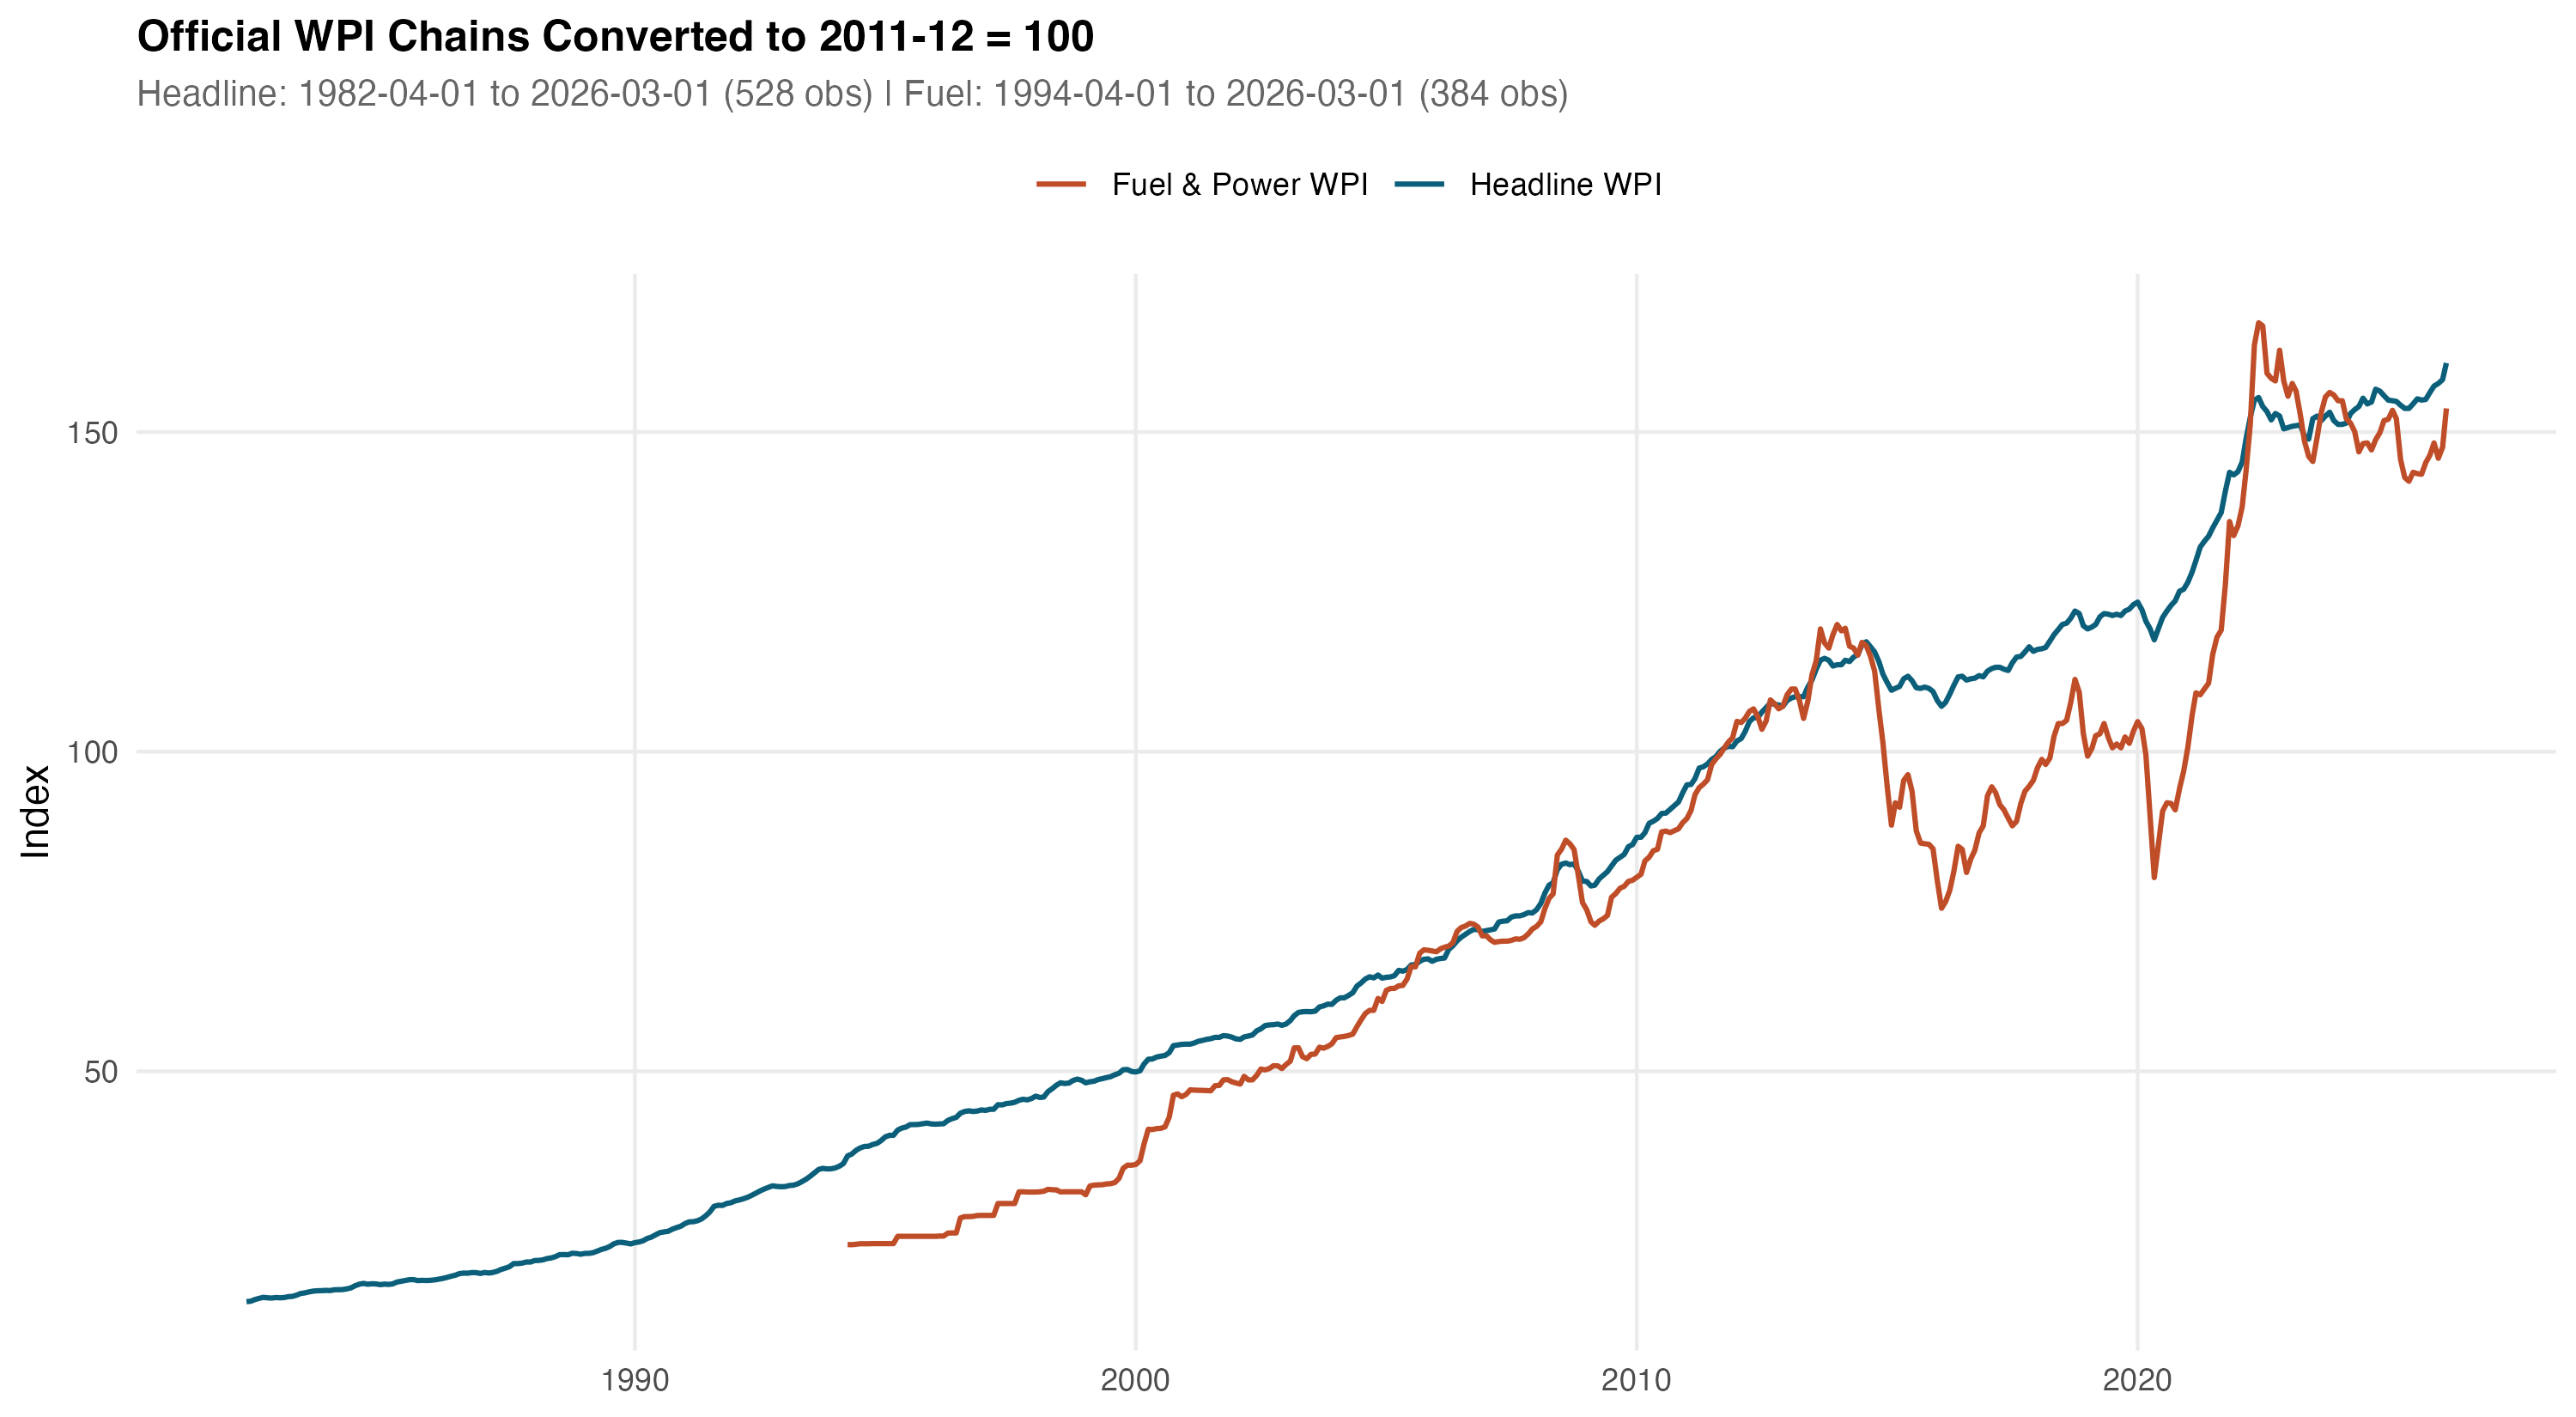
\includegraphics[width=0.88\linewidth]{fig_01_wpi_chained_series.png}
\caption{Chained WPI series, 2011-12 = 100. Headline WPI runs from April 1982 (528 monthly observations); Fuel \& Power begins April 1994 (384 observations). Splice points across the four official OEA base years are marked.}
\label{fig:chain}
\end{figure}

\begin{figure}[t]
\centering

\includegraphics[width=0.88\linewidth]{fig_03_oil_decomposition.png}
\caption{Decomposition of the rupee oil price into Brent (USD) and the INR/USD rate. Plotted in log levels with each series indexed to its January 2000 value. The two cost-side drivers move out of phase in some windows (notably 2003--2008 and 2014--2016), which is the variation the Brent + EXR robustness specification in Section \ref{sec:rob} exploits.}
\label{fig:decomp}
\end{figure}

All series are converted to month-on-month log differences. Let $\Delta y_t = \ln Y_t - \ln Y_{t-1}$ and $\Delta x_t = \ln X_t - \ln X_{t-1}$ where $X_t$ denotes the relevant oil measure. The asymmetric oil change is decomposed into a positive and a negative part:
\begin{equation}
\Delta x_t^+ = \max(\Delta x_t,0), \qquad \Delta x_t^- = \min(\Delta x_t,0).
\end{equation}
The main estimating equation is the short-run asymmetric ADL
\begin{equation}
\Delta y_t = \alpha + \sum_{i=1}^{12} \phi_i \Delta y_{t-i} + \sum_{j=0}^{6} \beta_j^+ \Delta x_{t-j}^+ + \sum_{j=0}^{6} \beta_j^- \Delta x_{t-j}^- + \gamma' Z_t + \mu_m + u_t,
\label{eq:adl}
\end{equation}
where $Z_t$ collects controls (notably $\Delta \ln \mathrm{EXR}_t$ in the Brent decomposition), $\mu_m$ are calendar-month fixed effects, and $u_t$ is an error process whose autocorrelation we accommodate through Newey--West standard errors with a Bartlett kernel and Newey--West lag truncation. The cumulative pass-through summaries are
\begin{equation}
\mathrm{CPT}^+ = \sum_{j=0}^{6} \beta_j^+, \qquad \mathrm{CPT}^- = \sum_{j=0}^{6} \beta_j^-,
\end{equation}
with significance assessed using HAC Wald tests on the linear restrictions $\mathrm{CPT}^+ = 0$, $\mathrm{CPT}^- = 0$ and the symmetry restriction $\mathrm{CPT}^+ = \mathrm{CPT}^-$. For the symmetry test we also report a finite-sample $p$-value from a restricted-residual circular block bootstrap with 4{,}999 replications.

The choice of an ADL in differences rather than a NARDL in levels is deliberate. Standard unit-root tests reject I(1) for all the differenced series we use; ADF and Phillips--Perron statistics on $\Delta \ln \mathrm{WPI}$ are $-12.22$ and $-14.39$. KPSS gives a borderline rejection of stationarity for $\Delta \ln \mathrm{WPI}$ ($\hat\eta = 0.90$ against a 5\% critical value of $0.46$), which we read as a known KPSS over-rejection in long samples with structural breaks rather than as evidence of a unit root in the differences \citep[see][]{rbi2014}. A Bai--Perron break test finds one break in $\Delta \ln \mathrm{WPI}$ at September 2013, which is the disinflationary regime change familiar from the inflation-targeting transition. With this in mind, ADL in differences with Newey--West inference is the cleaner short-run vehicle. We retain a NARDL-in-levels battery in the appendix for two reasons: it provides a long-run cointegration check, and it is the dominant method in the Indian pass-through literature, so silence on it would be conspicuous.

The retail-fuel mechanism model uses $\Delta \ln \mathrm{Petrol}_t^{\text{Delhi}}$ as the dependent variable and asymmetric Brent (in USD) as the regressor, with $q = 3$ lags on each side. Although the petrol pricing regime moved to fortnightly in 2014 and to daily revisions in 2017, monthly averaging is appropriate for the cross-layer comparison and avoids the Brent--EXR averaging mismatch that a daily specification would inherit. The CPI bridge model regresses $\Delta \ln \mathrm{Fuel\&Light}^{\text{CPI}}_t$ on asymmetric retail petrol changes; this is reported as a bridge equation only because the available CPI Fuel and Light series begins in May 2011 and falls below the 20-year window we treat as the minimum sample for headline mandates.

Granger predictive precedence is reported alongside the ADL evidence as a complementary check. We treat Granger statistics as evidence of lead--lag predictability rather than of structural causality, in line with the conservative reading common in the recent literature.

\section{Historical wholesale pass-through}
\label{sec:wpi}

We start with the longest sample. Table \ref{tab:wpi} reports the headline WPI ADL on rupee oil for May 1983 through March 2026 ($N=515$, span 42.92 years).

\begin{table}[t]
\centering
\caption{Headline WPI ADL on rupee oil. Cumulative pass-through over lags 0--6.}
\label{tab:wpi}
\footnotesize
\setlength{\tabcolsep}{5pt}
\begin{threeparttable}
\begin{tabular}{l c c c c c c}
\toprule
Specification & $N$ & Span (yrs) & Adj.\ $R^2$ & CPT$^+$ & CPT$^-$ & Asym.\ $p$ \\
\midrule
Headline WPI ADL, INR oil & 515 & 42.92 & 0.421 & 0.030 & 0.037 & 0.673 \\
$p$-value on cumulative coefficient & & & & 0.024 & 0.001 & \\
\midrule
\multicolumn{7}{l}{\emph{Bootstrap symmetry} ($B = 4{,}999$, restricted-residual circular block):} \\
Bootstrap $p$ on CPT$^+$ = CPT$^-$ & & & & & & 0.746 \\
\bottomrule
\end{tabular}
\begin{tablenotes}\footnotesize
\item Notes: Sample 1983-05 to 2026-03. Specification: $\Delta \ln \mathrm{WPI}_t$ on twelve own lags, lags 0--6 of $\Delta \ln \mathrm{Oil^{INR}}_t^{+}$ and $\Delta \ln \mathrm{Oil^{INR}}_t^{-}$, and calendar-month fixed effects. Newey--West HAC standard errors. Cumulative pass-through CPT$^\pm$ is the sum of the corresponding seven coefficients. Asymmetry $p$ is the HAC Wald test of CPT$^+$ = CPT$^-$.
\end{tablenotes}
\end{threeparttable}
\end{table}


\begin{figure}[t]
\centering
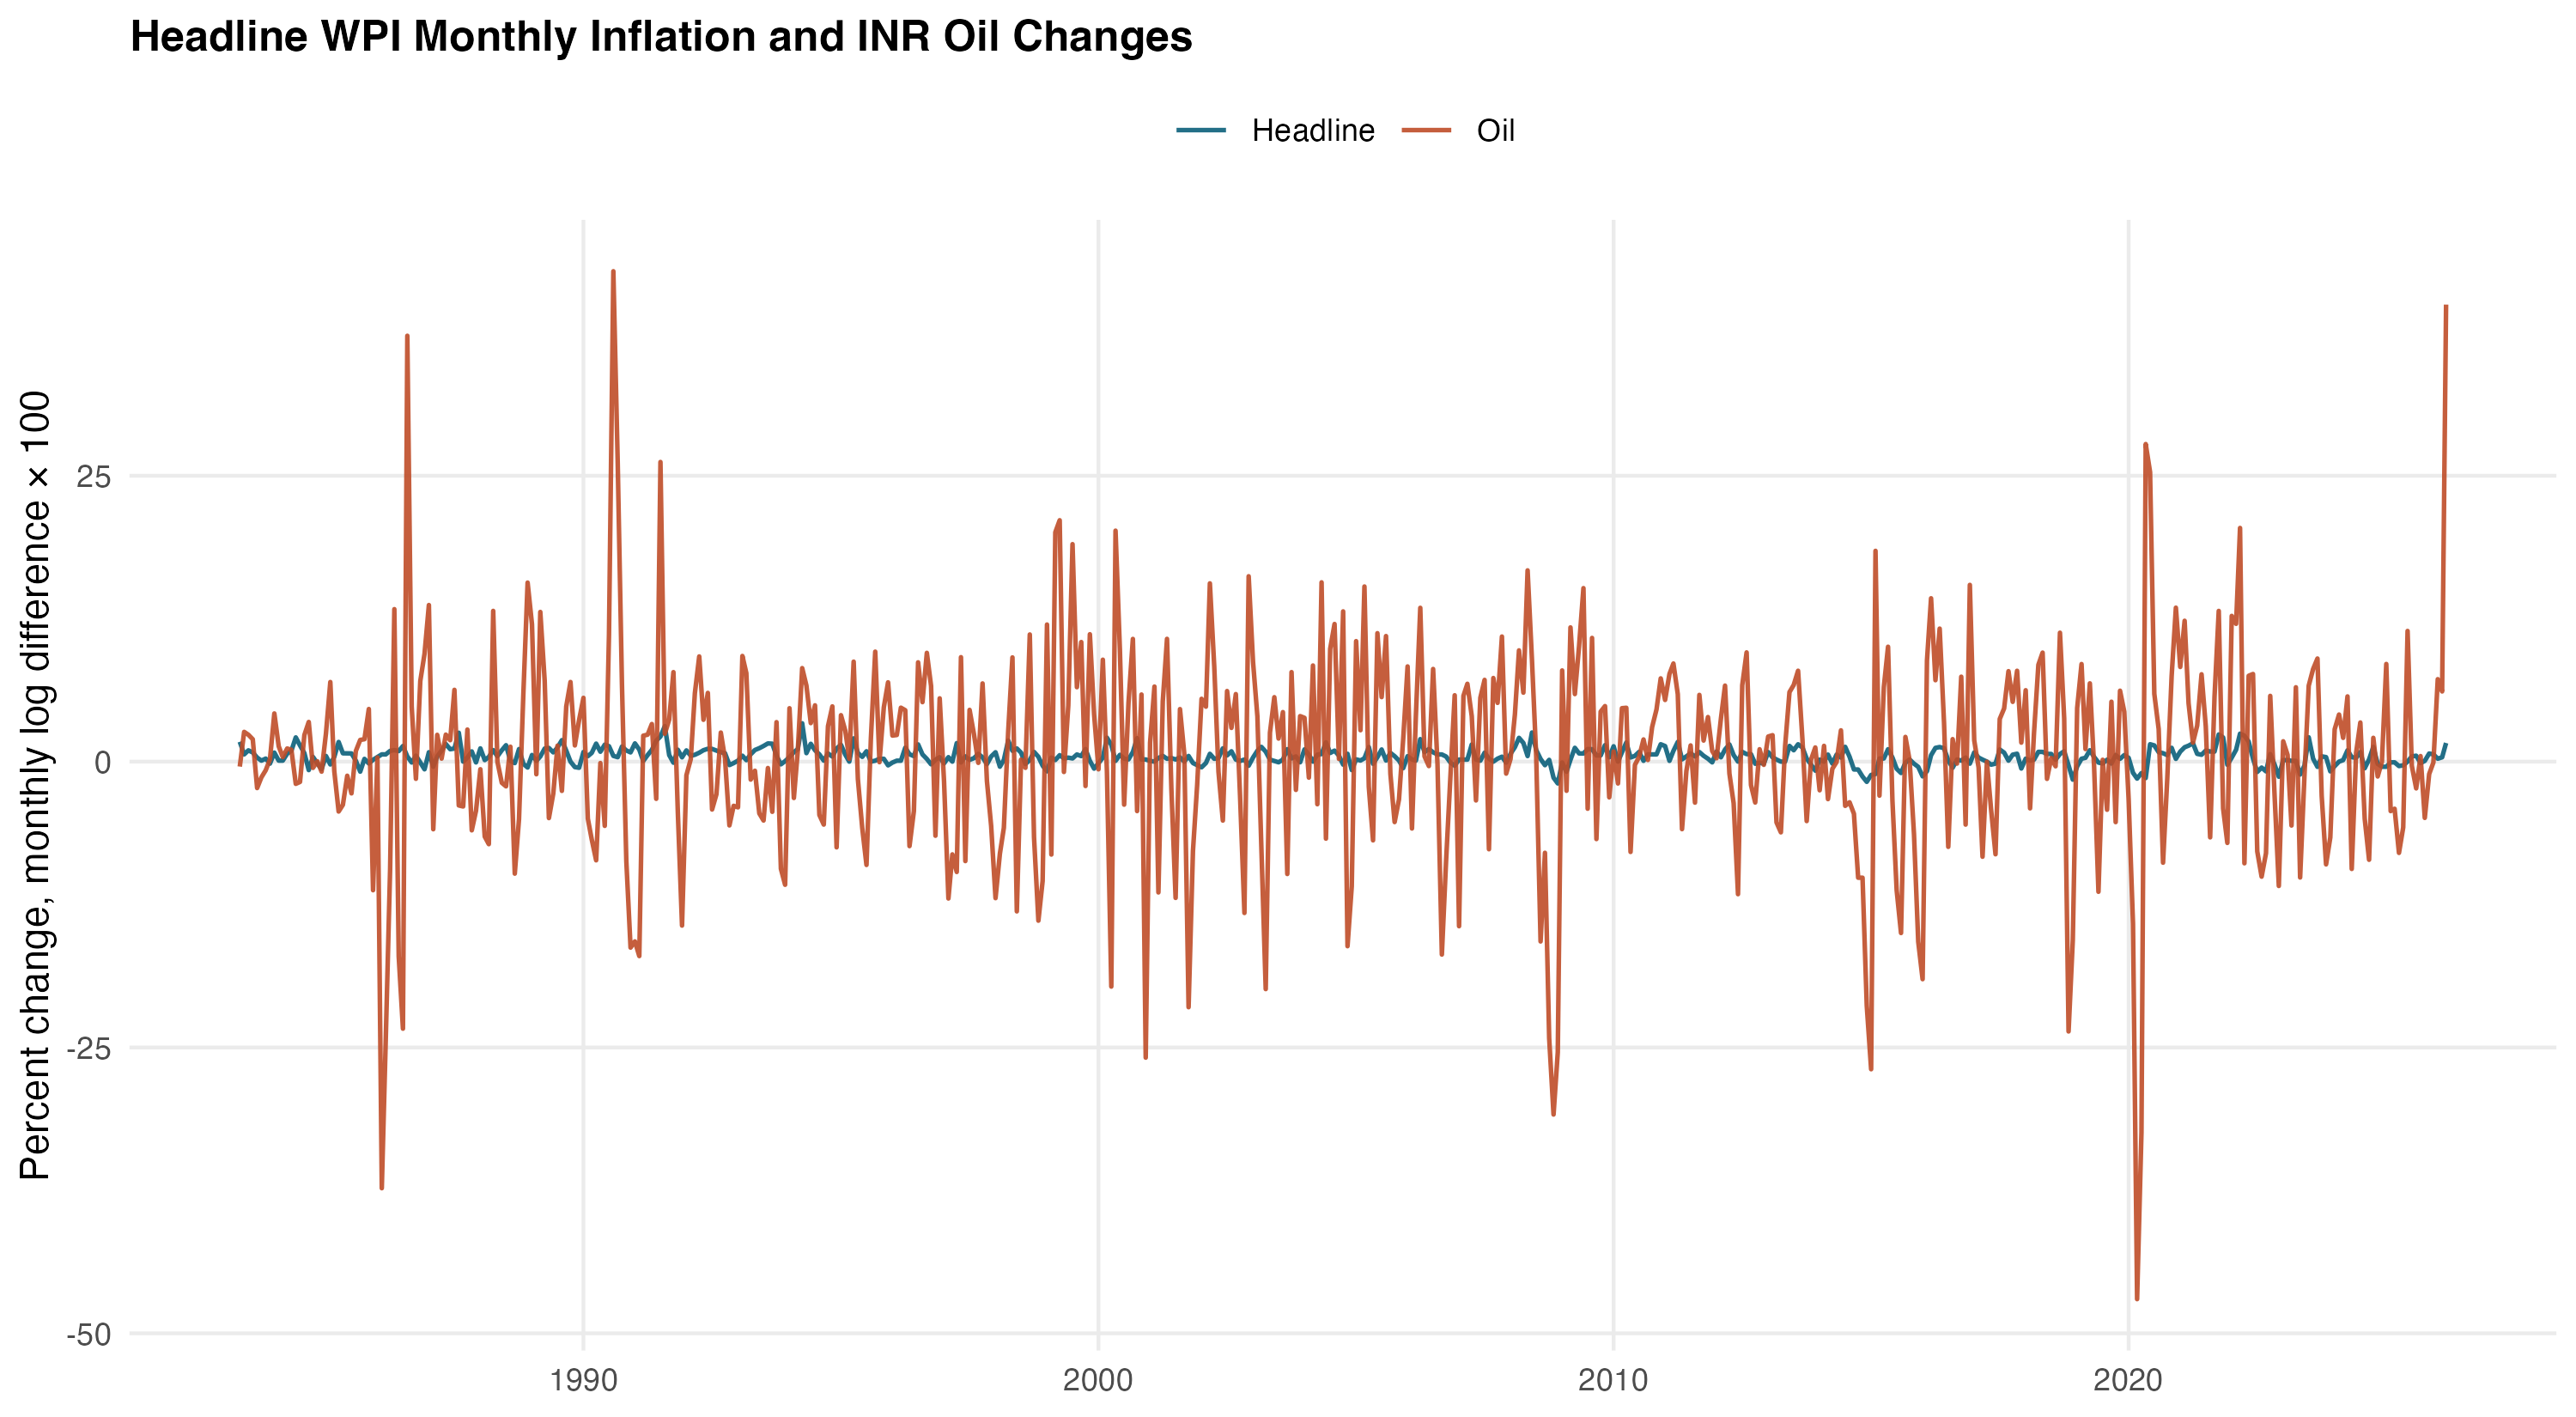
\includegraphics[width=0.92\linewidth]{fig_02_headline_inflation_vs_oil.png}
\caption{Headline WPI inflation and the rupee oil change, monthly, 1983--2026. Both series are plotted in $\Delta \ln$ form. The wholesale series tracks the rupee oil change visibly through the 1990s and from 2010 onward, with a quieter middle period that the subsample split picks up.}
\label{fig:wpi_oil}
\end{figure}

The picture is consistent across the two cumulative summaries. Positive oil shocks raise wholesale inflation by 3.0 percent of the shock over the seven-month window, with $p = 0.024$. Negative shocks subtract 3.7 percent, with $p = 0.001$. Both numbers are small but precise. The Wald symmetry test on the seven-lag restriction yields an asymptotic $p$-value of $0.673$ and a bootstrap $p$-value of $0.746$; the data give no support to short-run asymmetry over the full historical sample. The Brent + EXR decomposition (reported in the next section as a robustness check) returns a near-identical CPT$^+$ of $0.031$ and CPT$^-$ of $0.037$, which suggests that the rupee oil aggregate is not hiding a sign-cancelling combination of price and exchange-rate movements. Adjusted $R^2$ for the headline ADL is $0.42$. A Breusch--Godfrey test at twelve lags returns $p = 0.84$. The HAC RESET test passes ($p = 0.35$). The recursive CUSUM test passes at conventional levels ($p = 0.39$).

\begin{figure}[h]
\centering

\includegraphics[width=0.85\linewidth]{fig_04_cumulative_passthrough.png}
\caption{Cumulative pass-through profile for the headline WPI ADL. Lag-by-lag accumulation of the positive and negative rupee-oil coefficients from lag 0 through lag 6, with HAC bands. Most of the response is loaded onto the first three lags; the seven-lag sum stabilises at the values reported in Table \ref{tab:wpi}.}
\label{fig:cpt}
\end{figure}

The interesting result is the subsample split. Indian petrol prices were deregulated in June 2010 and diesel in October 2014. We split the sample at April 2010 to run a clean comparison and re-estimate the same ADL on the two windows.

\begin{table}[t]
\centering
\caption{Pre/post-2010 subsample comparison. Headline WPI and Fuel \& Power ADL.}
\label{tab:subsample}
\footnotesize
\setlength{\tabcolsep}{5pt}
\begin{threeparttable}
\begin{tabular}{l l c c c c c}
\toprule
Model & Subsample & $N$ & CPT$^+$ & $p$ & CPT$^-$ & $p$ \\
\midrule
Headline WPI ADL & Pre-2010 (1983-05 to 2010-03) & 323 & 0.012 & 0.381 & 0.025 & 0.043 \\
Headline WPI ADL & Post-2010 (2010-04 to 2026-03) & 192 & 0.074 & 0.004 & 0.081 & 0.000 \\
\midrule
Fuel \& Power ADL & Pre-2010 (1995-05 to 2010-03) & 179 & 0.092 & 0.168 & 0.238 & 0.000 \\
Fuel \& Power ADL & Post-2010 (2010-04 to 2026-03) & 192 & 0.524 & 0.000 & 0.438 & 0.000 \\
\bottomrule
\end{tabular}
\begin{tablenotes}\footnotesize
\item Notes: ADL specification as in Table \ref{tab:wpi}. Split point April 2010, the month after India's June 2010 petrol deregulation. The post-2010 window also contains the October 2014 diesel deregulation. The split should be read as descriptive of the post-deregulation regime and not as a causal identification of reform effects.
\end{tablenotes}
\end{threeparttable}
\end{table}


\begin{figure}[t]
\centering

\includegraphics[width=0.92\linewidth]{fig_05_subsample_comparison.png}
\caption{Pre/post-2010 subsample comparison of cumulative pass-through. Headline WPI and Fuel \& Power ADL specifications, plotted as cumulative coefficient response over lags 0--6. The post-2010 magnitudes are visibly larger across both panels, broadly consistent with the institutional shift toward market-linked transport-fuel pricing.}
\label{fig:subsample}
\end{figure}

The pre-2010 estimates are weak. Positive shocks pass through with CPT$^+ = 0.012$ ($p = 0.38$) and negative shocks with CPT$^- = 0.025$ ($p = 0.04$). After deregulation, the same model on the post-2010 sample returns CPT$^+ = 0.074$ ($p = 0.004$) and CPT$^- = 0.081$ ($p < 0.001$). The post-period magnitudes are roughly six times the pre-period magnitudes on the positive side and three times on the negative side. The fuel-and-power subindex tells the same story with larger magnitudes. Pre-2010 fuel CPT$^+$ is $0.092$ and not significant; post-2010 it jumps to $0.524$ and is highly significant. We read these comparisons as broadly consistent with the institutional shift toward more market-linked pricing, but we are deliberate about not calling them a causal identification of reform effects. The 2010--2014 window contains both monetary regime changes and global oil cycles, and the split-sample comparison cannot net these out cleanly.

Two stylised observations help frame what follows. First, even at its full-sample maximum, headline WPI pass-through is small in absolute terms: a one percent rupee oil rise lifts wholesale inflation by about three basis points cumulatively over seven months. Second, the absence of short-run asymmetry in the headline series sits in tension with the asymmetric findings reported by parts of the Indian NARDL literature \citep{abubakar2018,suresh2026}. We pick that tension up explicitly in Section \ref{sec:rob}, where the appendix NARDL battery does detect long-run asymmetry while the short-run ADL does not. The two methods are not contradictory. They are pricing different things. ADL in differences is asking whether the seven-month sum of positive coefficients matches the seven-month sum of negative coefficients. NARDL in levels is asking whether the long-run multipliers from positive and negative cumulative oil shocks differ. Long-run asymmetry can coexist with short-run symmetry. Our preference for the short-run reading in the body of the paper is partly a matter of inferential transparency. The bootstrap distribution for the symmetry test is well-behaved on the differenced specifications, and the standard errors do not require an assumed cointegration structure to be valid.

The long-horizon wholesale evidence, taken together, supports a moderate but credible historical pass-through. It also points to where the action sits in the more recent data. The next section turns to the layers in which the same shock shows up an order of magnitude larger.

\section{Mechanism and attenuation across layers}
\label{sec:mech}

The point of the integrated design is in this section. We move along the chain from crude to consumer, and at each step we ask how much of the upstream signal is preserved.

Figure \ref{fig:map} sketches the chain we estimate. Brent and the rupee/dollar rate combine into the rupee oil price. The rupee oil price feeds into PPAC retail petrol at the pump. Retail fuel prices feed into the fuel-sensitive subindices of WPI (Fuel and Power) and CPI (Fuel and Light). The fuel-sensitive subindices, together with non-fuel cost pressures, feed into the two headline aggregates. The arrows in the diagram are weighted by the cumulative positive pass-through estimates from our ADL specifications. The CPI endpoint arrow is dashed and thinned to convey what the data say: by the time the shock reaches headline CPI, very little of it is left.

\begin{figure}[t]
\centering
\resizebox{\linewidth}{!}{%
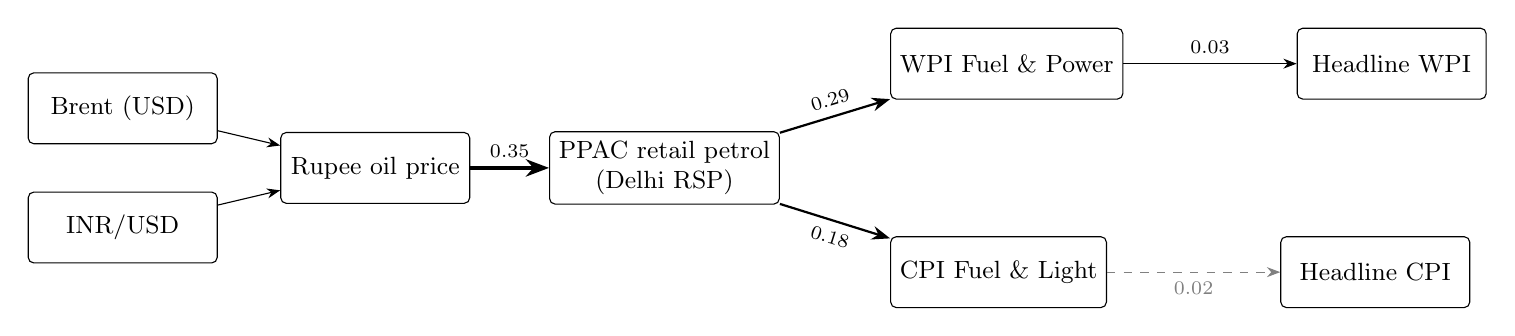
\begin{tikzpicture}[
  >=Stealth, node distance=6mm and 10mm,
  box/.style={draw, rounded corners=2pt, align=center, minimum width=24mm, minimum height=9mm, font=\small},
  small/.style={font=\scriptsize}]
  \node[box] (brent) {Brent (USD)};
  \node[box, below=of brent] (exr) {INR/USD};
  \node[box, right=20mm of $(brent)!0.5!(exr)$] (oilinr) {Rupee oil price};
  \node[box, right=of oilinr] (petrol) {PPAC retail petrol\\(Delhi RSP)};
  \node[box, above right=4mm and 14mm of petrol] (wpifp) {WPI Fuel \& Power};
  \node[box, below right=4mm and 14mm of petrol] (cpifl) {CPI Fuel \& Light};
  \node[box, right=22mm of wpifp] (wpi) {Headline WPI};
  \node[box, right=22mm of cpifl] (cpi) {Headline CPI};

  \draw[->] (brent) -- (oilinr);
  \draw[->] (exr) -- (oilinr);
  \draw[->, very thick] (oilinr) -- node[small,above]{0.35} (petrol);
  \draw[->, thick] (petrol) -- node[small,above,sloped]{0.29} (wpifp);
  \draw[->, thick] (petrol) -- node[small,below,sloped]{0.18} (cpifl);
  \draw[->] (wpifp) -- node[small,above]{0.03} (wpi);
  \draw[->, dashed, gray] (cpifl) -- node[small,below]{0.02} (cpi);
\end{tikzpicture}}
\caption{Conceptual transmission map. Edge labels are cumulative positive pass-through estimates (CPT$^+$) from the ADL specifications reported in Tables \ref{tab:wpi}--\ref{tab:cpi}. The headline CPI arrow is dashed to mark that the corresponding coefficient is not statistically distinguishable from zero.}
\label{fig:map}
\end{figure}

\subsection{Retail fuel and the wholesale fuel layer}

Table \ref{tab:mech} reports the two upstream mechanism models. Panel A is the PPAC Delhi retail petrol model on August 2004 to December 2024 ($N=245$). Panel B is the WPI Fuel and Power ADL on May 1995 to March 2026 ($N=371$).

\begin{table}[t]
\centering
\caption{Mechanism layer ADL models. Retail petrol and wholesale fuel.}
\label{tab:mech}
\footnotesize
\setlength{\tabcolsep}{5pt}
\begin{threeparttable}
\begin{tabular}{l c c c c c c}
\toprule
Specification & $N$ & Span (yrs) & Adj.\ $R^2$ & CPT$^+$ & CPT$^-$ & Asym.\ $p$ \\
\midrule
\multicolumn{7}{l}{\emph{Panel A. PPAC Delhi retail petrol on Brent (USD), $q = 3$:}} \\
$\Delta \ln \mathrm{Petrol}_t$ ADL & 245 & 20.42 & 0.236 & 0.346 & 0.191 & 0.100 \\
$p$-value on cumulative coefficient & & & & 0.000 & 0.000 & \\
\midrule
\multicolumn{7}{l}{\emph{Panel B. WPI Fuel \& Power on rupee oil:}} \\
$\Delta \ln \mathrm{Fuel\&Power}_t$ ADL & 371 & 30.92 & 0.463 & 0.287 & 0.268 & 0.783 \\
$p$-value on cumulative coefficient & & & & 0.000 & 0.000 & \\
\bottomrule
\end{tabular}
\begin{tablenotes}\footnotesize
\item Notes: Panel A sample 2004-08 to 2024-12. Panel B sample 1995-05 to 2026-03. Both panels report HAC (Newey--West) inference on the cumulative pass-through. Panel B includes a post-October-2014 diesel deregulation dummy and an April--September 2020 COVID dummy in addition to month fixed effects. The HAC RESET test fails on Panel B at $p < 0.001$ (see Section \ref{sec:rob}); other diagnostics pass.
\end{tablenotes}
\end{threeparttable}
\end{table}


The retail petrol response is the largest in the chain. CPT$^+ = 0.346$ ($p < 0.001$) and CPT$^- = 0.191$ ($p < 0.001$). Asymmetry is borderline ($p = 0.10$), with the asymmetry running in the conventional rockets-and-feathers direction: positive shocks are passed through faster and more fully than negative ones. This is the empirical signature most consistent with the descriptive picture of post-deregulation pump pricing in India. It is also broadly consistent with the magnitudes reported by \citet{deheri2024} and \citet{pradeep2022} for the petrol channel.

The fuel-and-power subindex of WPI sits one step downstream and shows comparable but slightly smaller magnitudes, with CPT$^+ = 0.287$ and CPT$^- = 0.268$ (both $p < 0.001$). Symmetry is not rejected here ($p = 0.78$), which we read as a sign that the wholesale fuel index aggregates retail and bulk pricing channels in a way that washes out the asymmetry visible at the pump. We flag one diagnostic caveat: HAC RESET fails ($p < 0.001$) on the fuel and power model, which is most likely picking up a non-linearity in the level relationship that the differenced specification cannot remove. We retain the model in the main results because the cumulative pass-through estimates are stable across alternative lag choices and across COVID-window sensitivity checks (reported in Section \ref{sec:rob}), but we treat the fuel and power equation as the more fragile of the two upstream models.

\subsection{The consumer endpoint}

Now move to the bottom of the chain. Table \ref{tab:cpi} reports the headline CPI ADL.

\begin{table}[t]
\centering
\caption{Headline CPI ADL on rupee oil. Consumer endpoint.}
\label{tab:cpi}
\footnotesize
\setlength{\tabcolsep}{5pt}
\begin{threeparttable}
\begin{tabular}{l c c c c c c}
\toprule
Specification & $N$ & Span (yrs) & Adj.\ $R^2$ & CPT$^+$ & CPT$^-$ & Asym.\ $p$ \\
\midrule
Headline CPI ADL, INR oil & 245 & 20.42 & 0.449 & 0.021 & 0.001 & 0.241 \\
$p$-value on cumulative coefficient & & & & 0.122 & 0.938 & \\
\midrule
\multicolumn{7}{l}{\emph{Selected covariate effects (HAC $t$-tests on the levels coefficients):}} \\
\multicolumn{2}{l}{Diesel deregulation step (October 2014)} & \multicolumn{2}{l}{$\hat\beta = -0.339$} & \multicolumn{2}{l}{$p < 0.001$} & \\
\multicolumn{2}{l}{Petrol deregulation step (June 2010)} & \multicolumn{2}{l}{$\hat\beta = +0.116$} & \multicolumn{2}{l}{$p = 0.307$} & \\
\multicolumn{2}{l}{COVID window (April--September 2020)} & \multicolumn{2}{l}{$\hat\beta = -0.345$} & \multicolumn{2}{l}{$p = 0.507$} & \\
\bottomrule
\end{tabular}
\begin{tablenotes}\footnotesize
\item Notes: Sample 2004-08 to 2024-12. Specification analogous to Table \ref{tab:wpi} with $q = 3$ on the asymmetric oil components, an IIP control for industrial activity, and step dummies for the petrol and diesel deregulation events. The bootstrap $p$-value on the symmetry restriction is $0.500$.
\end{tablenotes}
\end{threeparttable}
\end{table}


The headline CPI estimates are the smallest and the least precise in the chain. Positive shocks have CPT$^+ = 0.021$ with $p = 0.12$. Negative shocks are essentially flat: CPT$^- = 0.001$, $p = 0.94$. Symmetry is not rejected ($p = 0.24$). The bootstrap symmetry $p$-value is similar at $0.50$. Two readings are possible. One is that headline CPI in India is genuinely insulated from oil shocks because the CPI basket is heavily food-weighted, with combined food and beverage weights close to half of the index. The other is that the consumer fuel and tax buffers absorb much of what does come through. Both are likely true, and the data do not let us cleanly separate them.

What the data do let us do is record one institutional fact that any policy reading should not lose. The October 2014 diesel-deregulation dummy in the headline CPI ADL is large and significant in the negative direction (estimate $-0.339$, $p < 0.001$). The October 2014 step is, of course, one event, and a single dummy cannot identify a structural channel. But the sign and magnitude are consistent with the institutional reading that diesel-tax revisions have at times moved in a direction that offsets, rather than reinforces, the international price signal in the consumer index.

\subsection{Putting it together}

Table \ref{tab:summary} stitches the four CPT$^+$ estimates into a single layered comparison and adds the pre/post-2010 split for the two wholesale models.

\begin{table}[t]
\centering
\caption{Integrated attenuation across price layers and pre/post-2010 split.}
\label{tab:summary}
\footnotesize
\setlength{\tabcolsep}{4pt}
\begin{threeparttable}
\begin{tabular}{l l r r r r}
\toprule
Layer & Dependent variable & $N$ & Span & CPT$^+$ & CPT$^+$ $p$ \\
\midrule
\multicolumn{6}{l}{\emph{Panel A. Layered cross-section (full available samples):}} \\
Retail fuel pump      & $\Delta \ln \mathrm{Petrol}^{\mathrm{Delhi}}_t$    & 245 & 20.4 yrs & 0.346 & 0.000 \\
Wholesale fuel        & $\Delta \ln \mathrm{WPI\ Fuel\&Power}_t$           & 371 & 30.9 yrs & 0.287 & 0.000 \\
Consumer fuel (bridge)& $\Delta \ln \mathrm{CPI\ Fuel\&Light}_t$           & 164 & 13.7 yrs & 0.178 & 0.002 \\
Wholesale headline    & $\Delta \ln \mathrm{WPI}_t$                        & 515 & 42.9 yrs & 0.030 & 0.024 \\
Consumer headline     & $\Delta \ln \mathrm{CPI}_t$                        & 245 & 20.4 yrs & 0.021 & 0.122 \\
\midrule
\multicolumn{6}{l}{\emph{Panel B. Pre/post-2010 split (wholesale models):}} \\
Headline WPI, pre-2010   & $\Delta \ln \mathrm{WPI}_t$           & 323 & 1983--2010 & 0.012 & 0.381 \\
Headline WPI, post-2010  & $\Delta \ln \mathrm{WPI}_t$           & 192 & 2010--2026 & 0.074 & 0.004 \\
Fuel \& Power, pre-2010  & $\Delta \ln \mathrm{Fuel\&Power}_t$   & 179 & 1995--2010 & 0.092 & 0.168 \\
Fuel \& Power, post-2010 & $\Delta \ln \mathrm{Fuel\&Power}_t$   & 192 & 2010--2026 & 0.524 & 0.000 \\
\bottomrule
\end{tabular}
\begin{tablenotes}\footnotesize
\item Notes: All entries are cumulative pass-through estimates from short-run asymmetric ADL specifications, summed over lags 0--$q$ on the relevant positive component. Panel A uses each layer's full active sample. The CPI Fuel \& Light bridge equation is shown for completeness only; its sample begins in 2011 and falls below the 20-year window we treat as the minimum for headline mandates.
\end{tablenotes}
\end{threeparttable}
\end{table}


\begin{figure}[t]
\centering
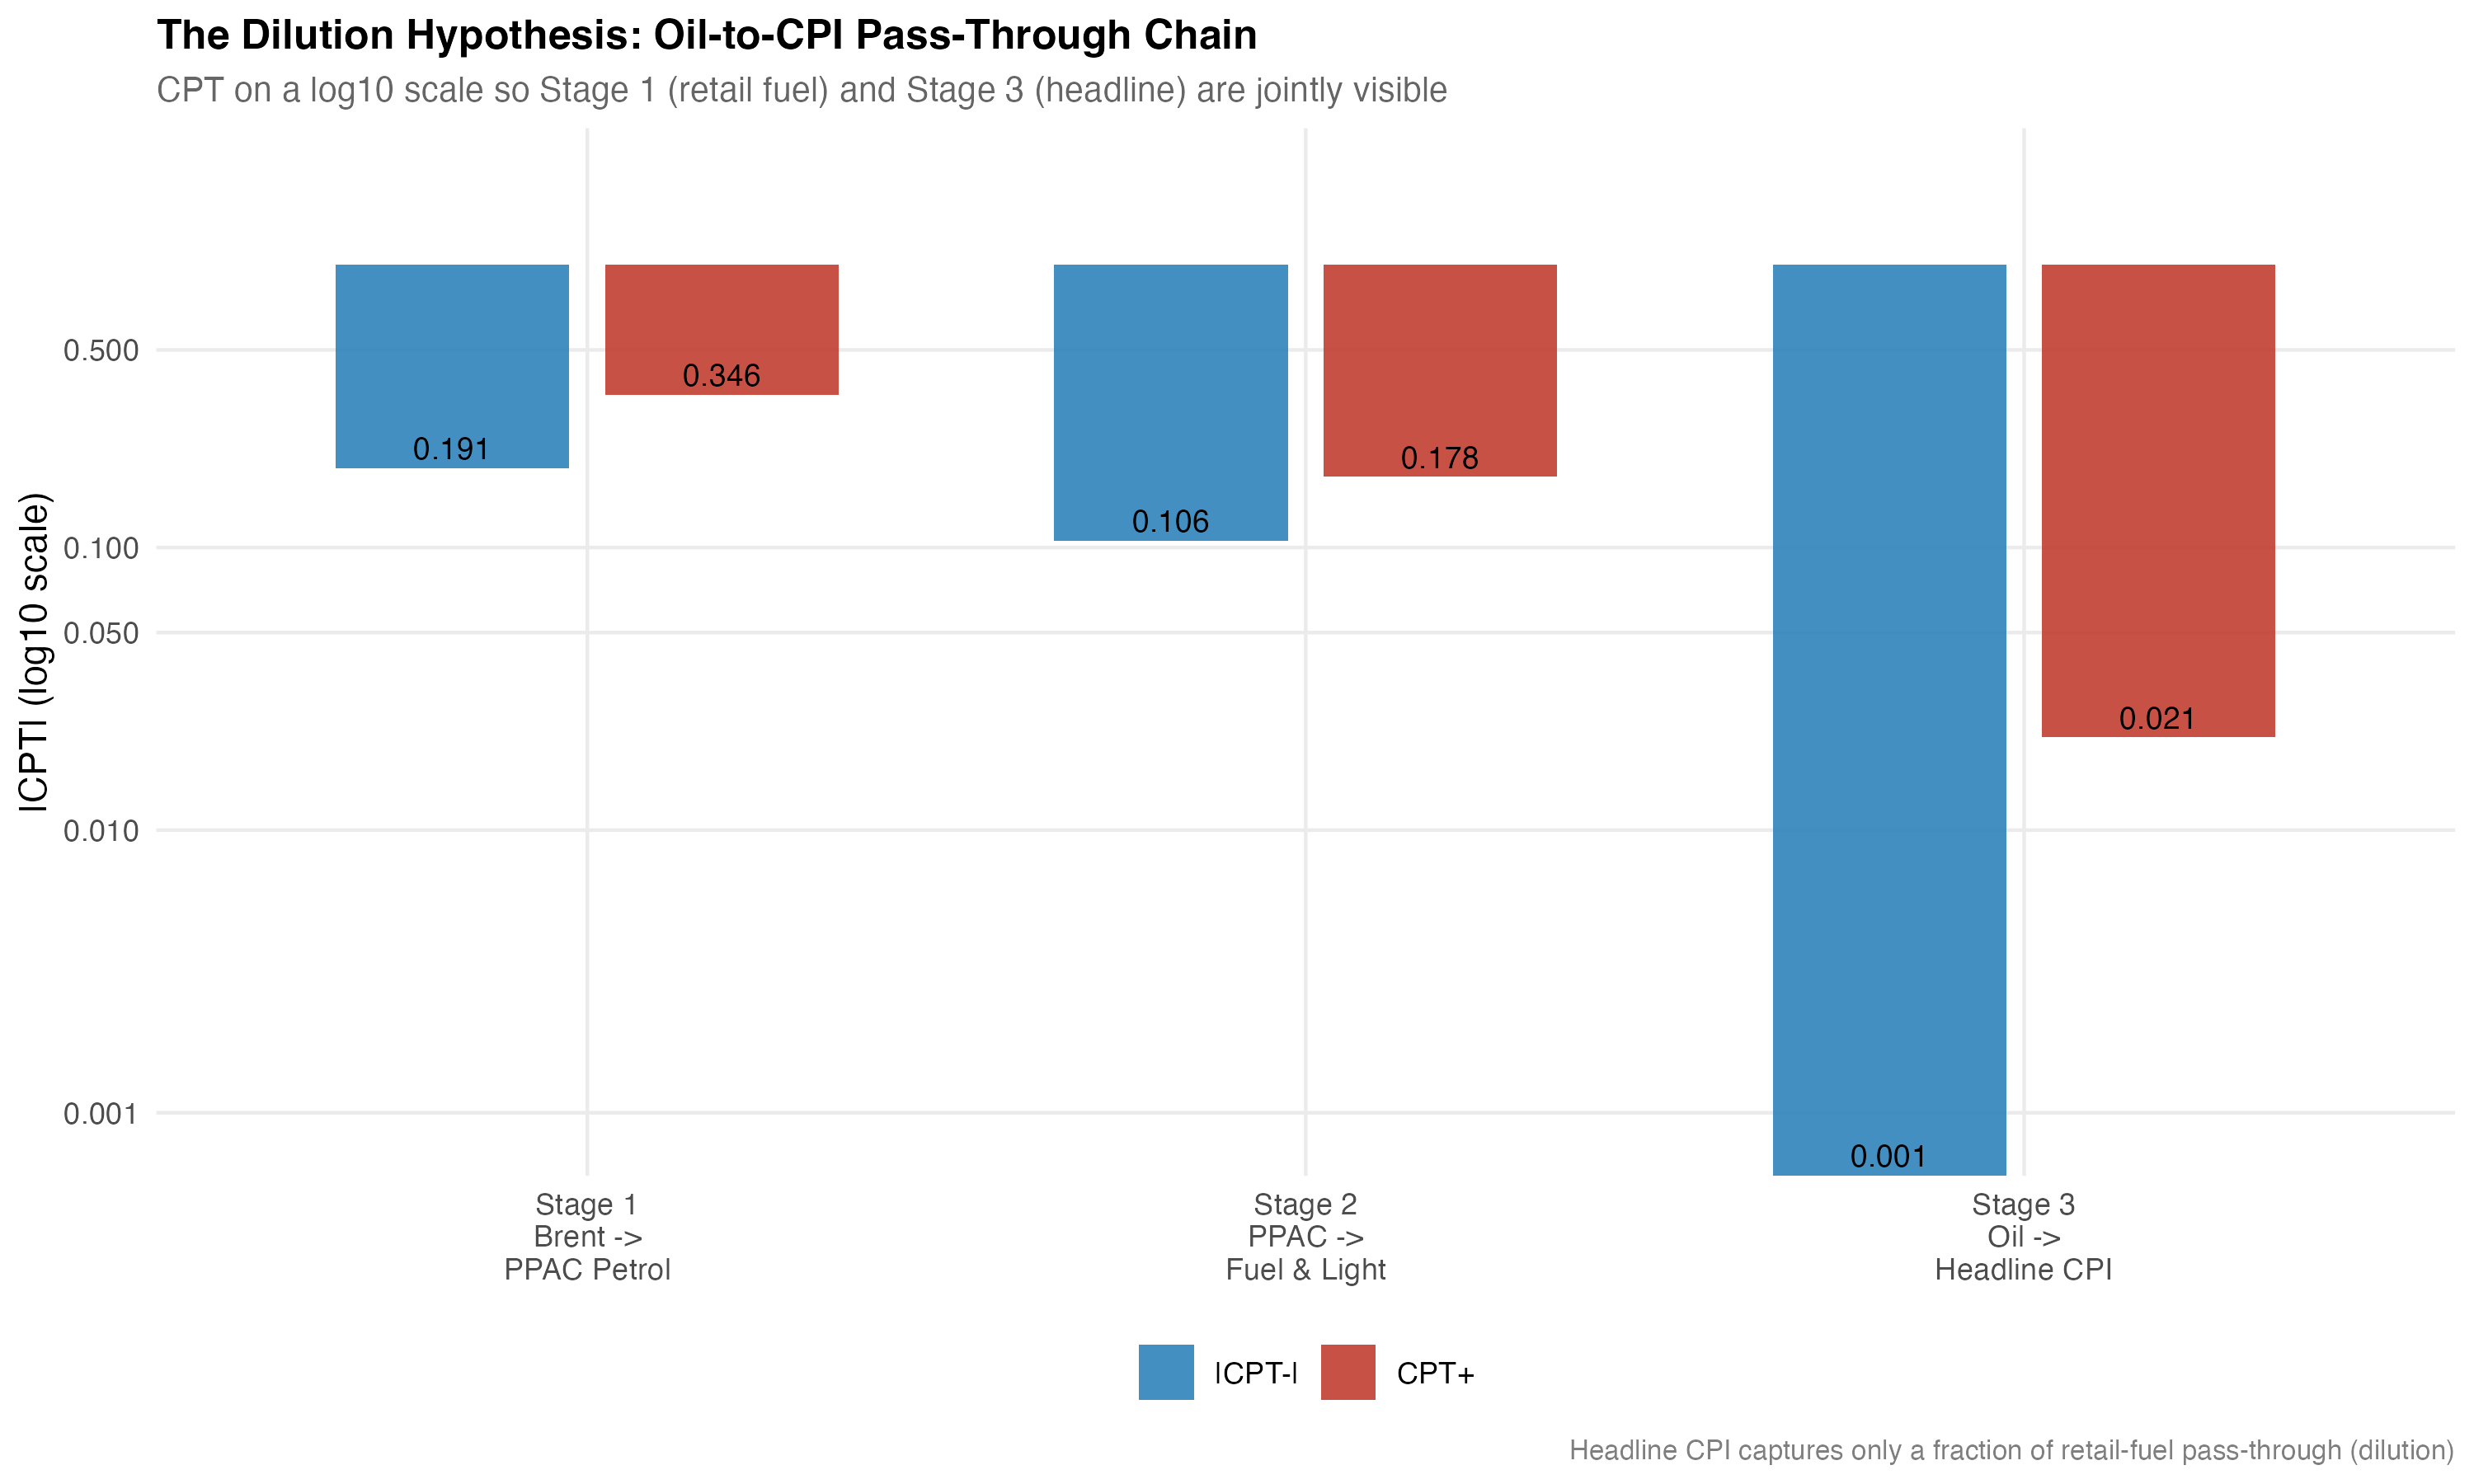
\includegraphics[width=0.92\linewidth]{fig_13_dilution_chain.png}
\caption{Attenuation across layers. Cumulative positive pass-through (CPT$^+$) by stage, from rupee oil through retail petrol, wholesale and consumer fuel-sensitive subindices, and the two headline aggregates. The headline-CPI bar is the smallest and is not statistically distinguishable from zero in the underlying ADL.}
\label{fig:attenuation}
\end{figure}

The picture is monotone in the obvious direction. Retail petrol has CPT$^+ = 0.35$. The two fuel-sensitive subindices come in at $0.29$ (WPI Fuel and Power) and $0.18$ (CPI Fuel and Light). Headline WPI is at $0.03$. Headline CPI is at $0.02$ and not significant. Roughly an order of magnitude is lost between the pump and the consumer. Most of that loss happens between the fuel-sensitive subindices and the headline aggregates, which is mechanical: fuel weights in the headline indices are small (about 13 percent in the WPI 2011--12 series and about 7 percent in the CPI 2010 base), so a large move in fuel cannot mathematically produce more than a small move in the aggregate unless non-fuel components correlate with it. The CPI Fuel and Light bridge equation, although it sits on a shorter sample (164 monthly observations beginning May 2011 and therefore not eligible as a headline mandate), confirms the qualitative direction: PPAC petrol passes into CPI Fuel and Light with CPT$^+ = 0.178$ ($p = 0.002$) and a smaller negative-side response.

\begin{figure}[h]
\centering
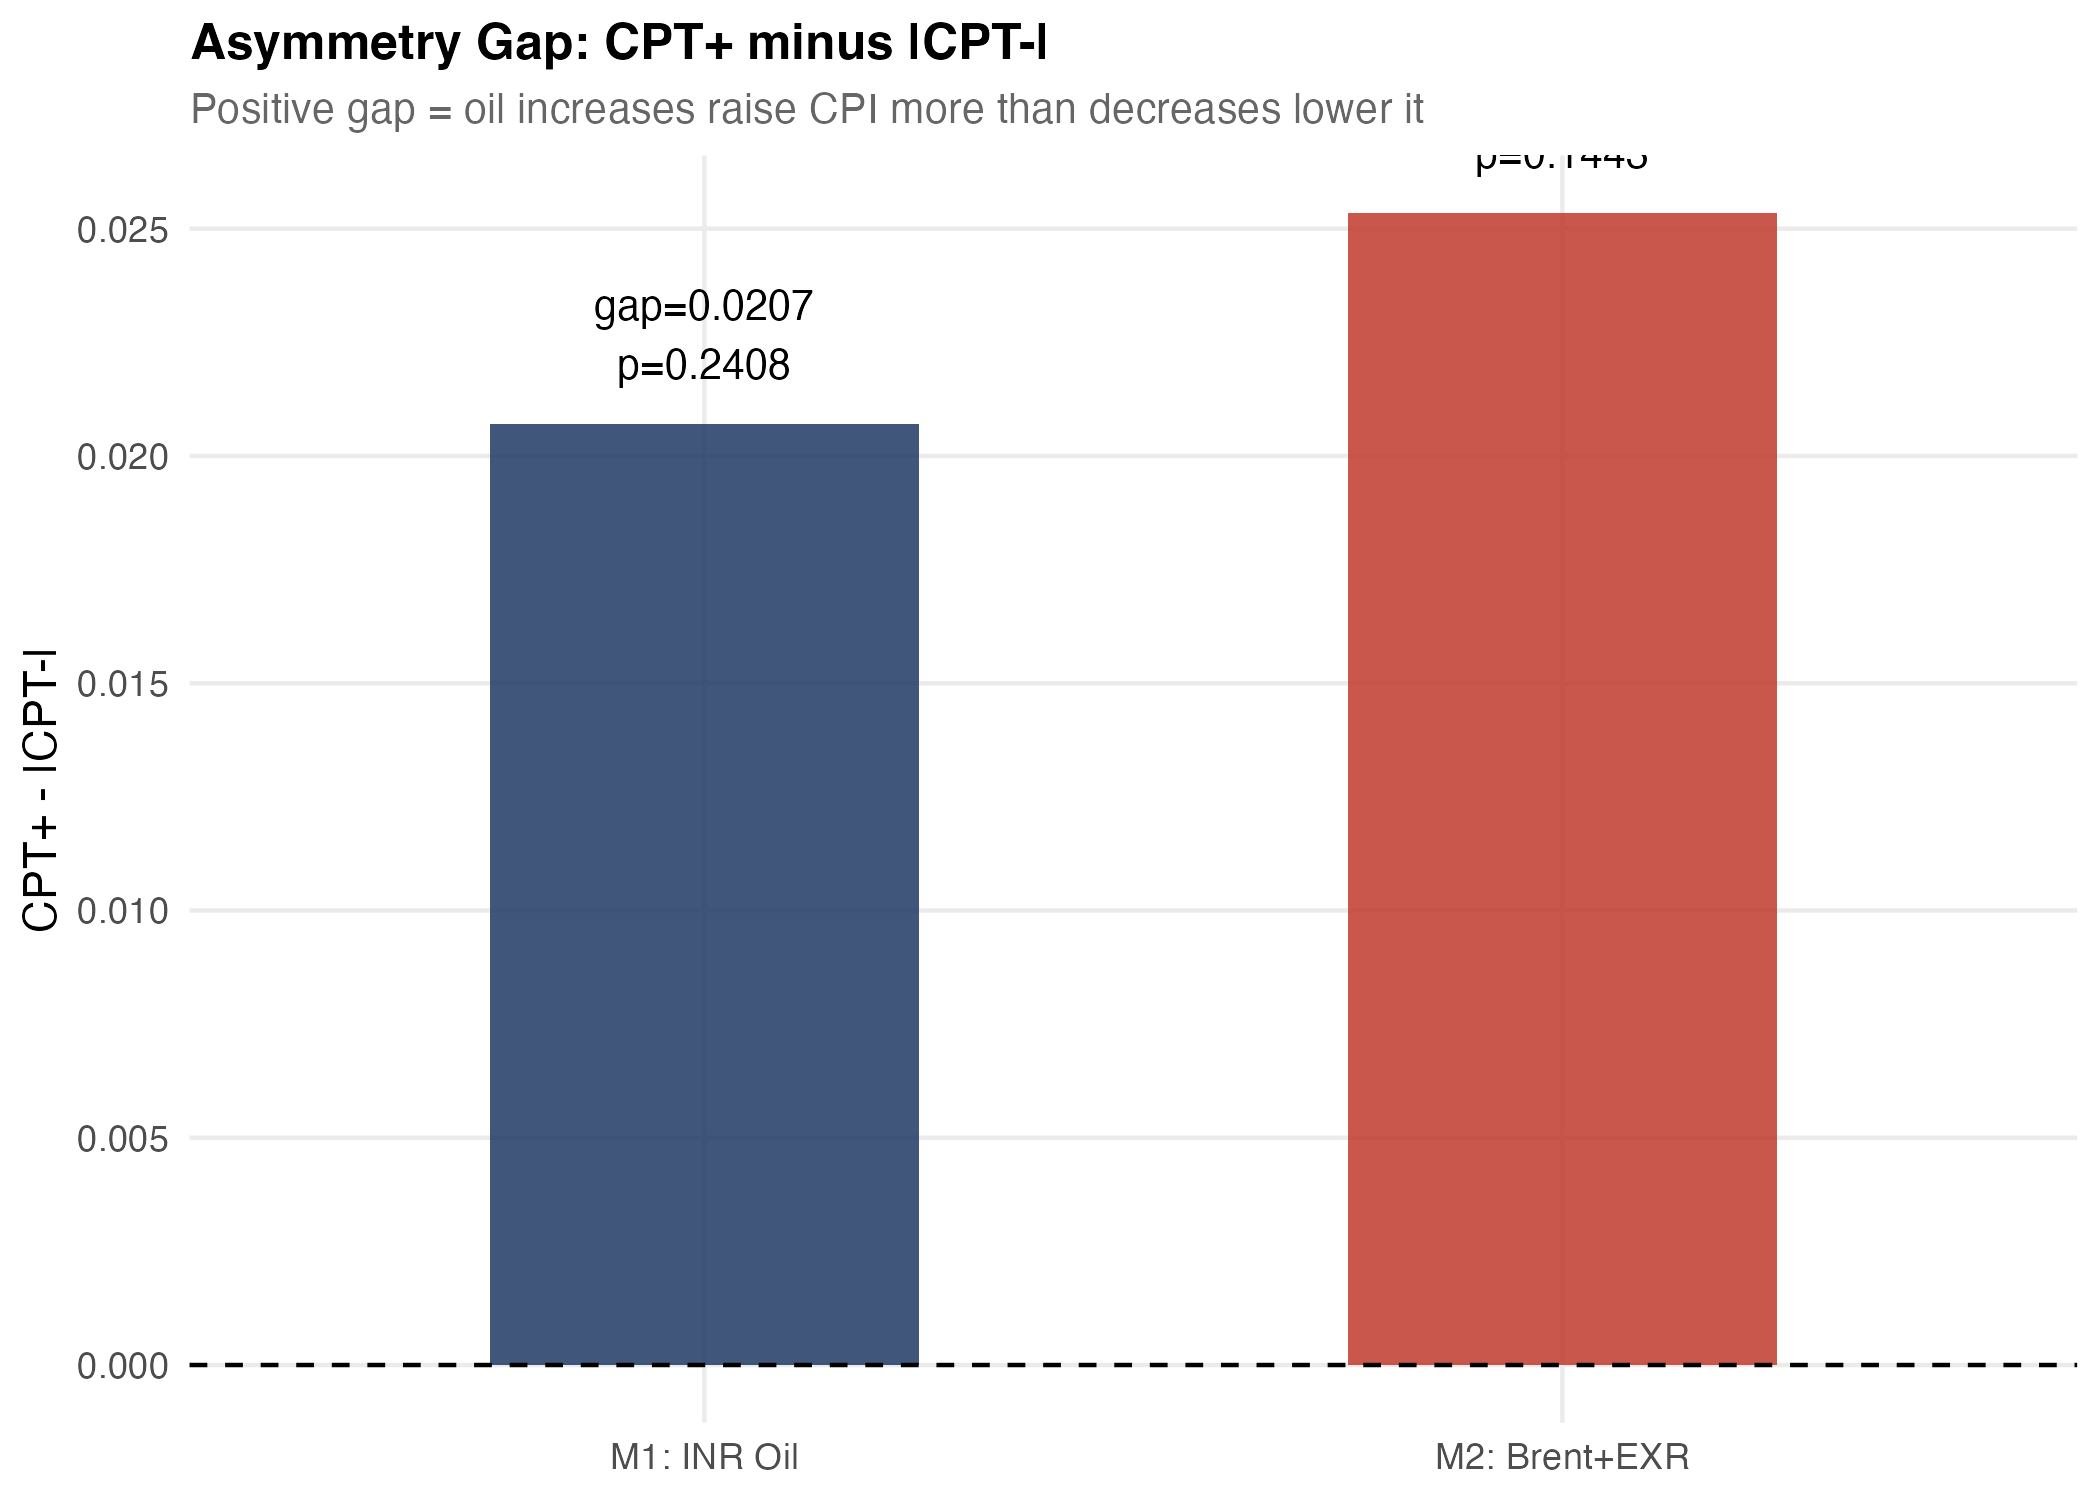
\includegraphics[width=0.85\linewidth]{fig_10_asymmetry_gap.png}
\caption{Asymmetry gap (CPT$^+$ minus CPT$^-$) by layer with HAC confidence bands. The gap is largest and signed positive at the retail-petrol stage, consistent with the conventional rockets-and-feathers reading. Both upstream-wholesale and headline-CPI gaps straddle zero.}
\label{fig:asymgap}
\end{figure}

We pick out one judgement call. The evidence here is more cautious about asymmetry than the recent Indian NARDL literature, which often headlines asymmetric long-run multipliers as the primary result. We do find asymmetry signals, but they are concentrated at the pump, are borderline at conventional significance ($p = 0.10$), and are not robust to moving up the chain. The integrated reading is that the most stable and quantitatively meaningful empirical feature in this dataset is attenuation across layers, not asymmetry within any single layer.

\FloatBarrier

\section{Robustness and supplementary evidence}
\label{sec:rob}

Three robustness exercises support the main reading.

First, the Brent + EXR decomposition. Replacing rupee oil with separate asymmetric Brent components and a contemporaneous EXR control yields CPT$^+ = 0.031$ ($p = 0.023$) and CPT$^- = 0.037$ ($p = 0.001$) on the headline WPI sample. Adjusted $R^2$ rises to $0.42$ and the symmetry test is not rejected ($p = 0.70$). The decomposition does not move the substantive conclusion, which suggests that the rupee oil aggregate used in the main specification is not masking offsetting movements in price and exchange rate components.

\begin{figure}[h]
\centering
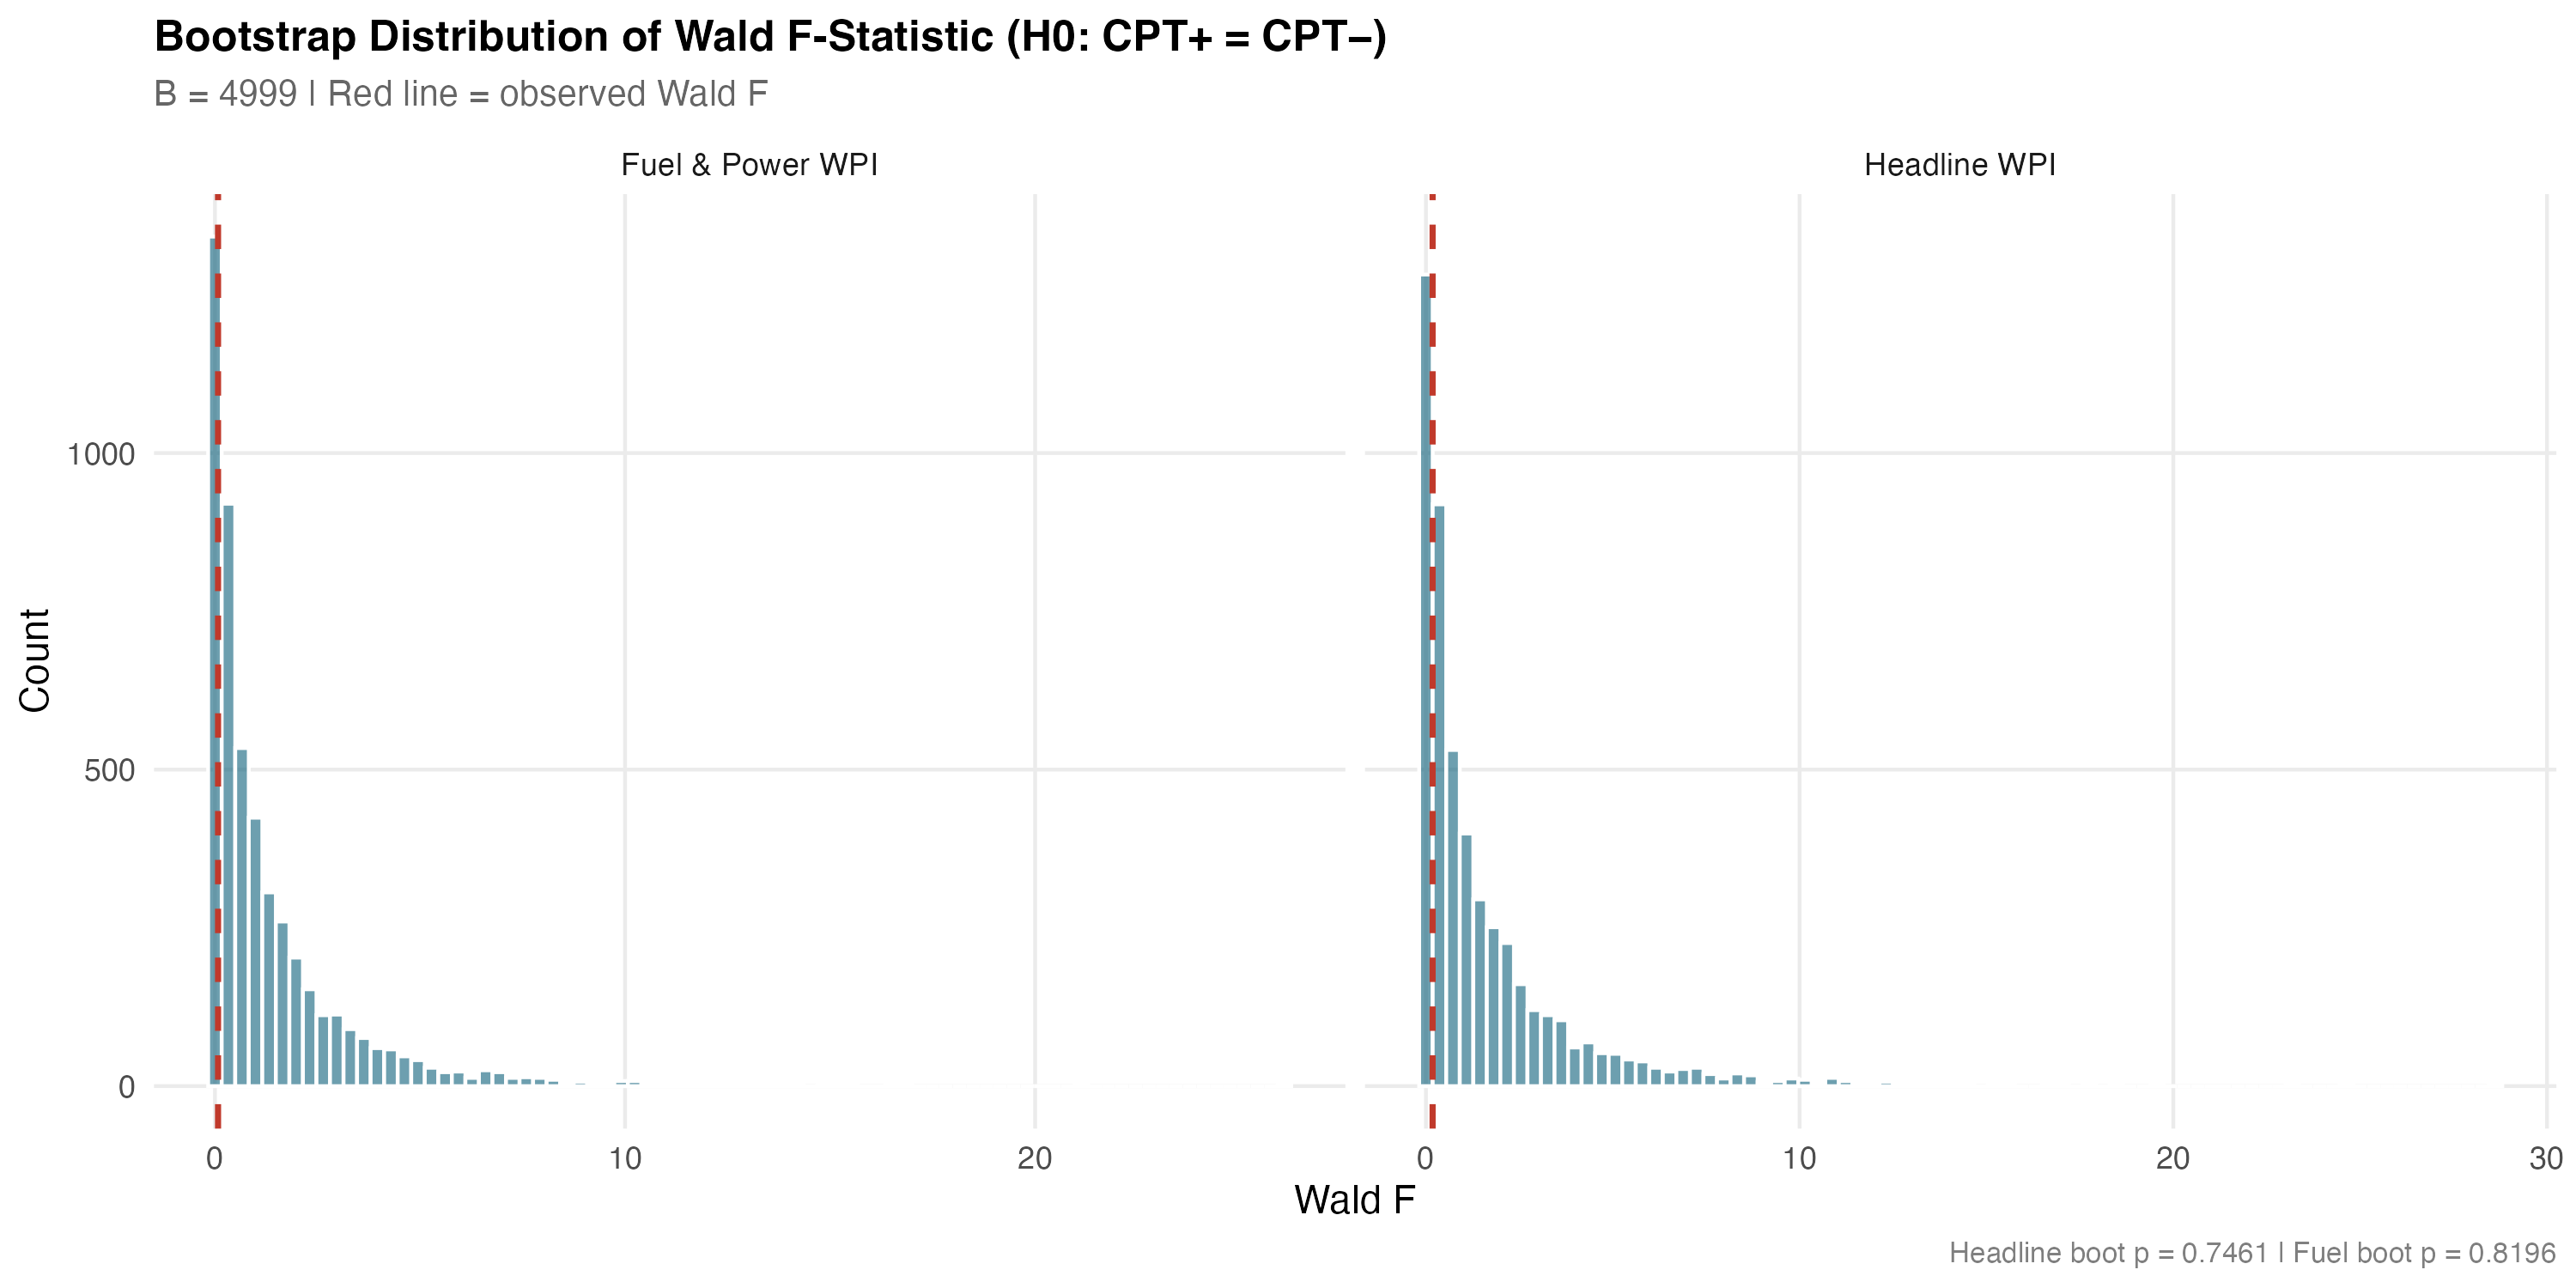
\includegraphics[width=0.85\linewidth]{fig_11_bootstrap_distribution.png}
\caption{Bootstrap distribution of the symmetry Wald statistic for the headline WPI ADL. Restricted-residual circular block bootstrap, $B = 4{,}999$. The observed Wald statistic sits near the centre of the simulated distribution, which gives a bootstrap symmetry $p$-value of $0.746$.}
\label{fig:boot}
\end{figure}

Second, the bootstrap symmetry tests. For both the headline WPI ADL and the WPI Fuel and Power ADL we resample residuals using a restricted-residual circular block bootstrap with 4{,}999 replications. The bootstrap symmetry $p$-values are $0.746$ for headline WPI and $0.820$ for fuel and power. There were no bootstrap failures. The asymptotic Wald conclusions hold up in finite samples on the wholesale models. The headline CPI bootstrap $p$-value is $0.50$, also consistent with the asymptotic test.

Third, predictive precedence. Granger tests at four lags reject the null of no Granger causation from rupee oil to headline WPI ($F = 7.43$, HAC $p < 0.001$), from rupee oil to WPI Fuel and Power ($F = 15.22$, HAC $p < 0.001$), and from Brent in USD to headline WPI ($F = 7.38$, HAC $p < 0.001$). The reverse direction is not Granger-significant for headline WPI ($p = 0.43$). The exchange rate Granger-causes WPI at the 10\% margin ($p = 0.05$). We treat these statistics as predictive precedence rather than as structural identification, in the conservative reading we adopt throughout.

\begin{figure}[h]
\centering

\includegraphics[width=0.85\linewidth]{fig_06_cusum_stability.png}
\caption{Recursive and OLS-CUSUM stability tests for the headline WPI ADL. Both test statistics stay inside their 5\% bands across the 1983--2026 sample, consistent with parameter stability in the differenced specification despite the September 2013 break detected by the Bai--Perron test on the dependent variable.}
\label{fig:cusum}
\end{figure}

A few sensitivity exercises round out the picture. Excluding the April--September 2020 COVID window does not materially change any of the headline pass-through estimates. Lag-sensitivity exercises moving the oil lag length between $q = 4$ and $q = 8$ leave the qualitative ranking of CPT$^+$ across layers intact. Winsorising the rupee oil change at the 1st and 99th percentiles trims the negative-side coefficient for the WPI Fuel and Power model slightly but does not alter the conclusion.

The appendix battery of NARDL bounds models in levels gives the long-run perspective. All four NARDL specifications reject the no-cointegration null at the 1\% upper bound of \citet{pesaran2001}. Each specification has a negative and significant error-correction coefficient. The long-run asymmetry tests of \citet{shin2014} reject equality of long-run positive and negative multipliers in three of four specifications, with the headline INR-oil specification on the borderline ($p = 0.023$). The fuel and power specification has the largest ECT magnitude (-0.081, $p < 0.001$), which is consistent with the higher pass-through speed in that layer that the ADL also picks up. We read the appendix NARDL evidence as supplementary. It identifies asymmetry that the differenced ADL does not. But the long-run multiplier estimates are sensitive to the assumed lag structure and to the unit-root status of the level series, and we do not want the appendix tail to wag the main-text dog.

The diagnostics are not uniformly clean. The WPI Fuel and Power ADL fails the HAC RESET test at $p < 0.001$. We have already flagged this. It is the model in which we would invest least in the precise point estimate, and it is one of two models for which the structural-break literature suggests the differenced specification still leaves curvature on the table. The headline WPI ADL passes Breusch--Godfrey at $p = 0.84$, RESET at $p = 0.35$ and recursive CUSUM at $p = 0.39$. The headline CPI ADL passes its diagnostics. The bootstrap symmetry tests, taken together with the diagnostics, support the central empirical claim: the magnitudes of the upstream pass-through estimates are credible, the headline-CPI weakness is not an artefact, and the cross-layer attenuation pattern is the robust feature of the data.

\section{Conclusion}
\label{sec:conc}

This paper has read Indian oil pass-through as a chain rather than as a single number. The chain begins with the rupee value of imported crude, runs through retail petrol pricing at the pump, into the fuel-sensitive subindices of the wholesale and consumer price indices, and out at the headline aggregates that policy targets. The transmission is uneven. It is large at the pump (cumulative pass-through of about 0.35 for positive oil shocks). It is comparable in the wholesale fuel layer (0.29). It is moderate in the consumer fuel layer (0.18). And it is small to absent in the two headline aggregates (0.03 for WPI, 0.02 and not significant for CPI). The pre-2010 versus post-2010 contrast in the wholesale numbers is consistent with the institutional shift toward market-linked pricing of transport fuels. Short-run asymmetry is detectable at the pump but is not robust as a feature of the headline pass-through. The supplementary NARDL evidence in the appendix recovers long-run asymmetry, which is consistent with parts of the recent literature, but we treat it as secondary to the integrated transmission story.

A few policy readings follow. WPI is more informative about upstream cost transmission and imported input pressures, while CPI is more informative about household-facing inflation. Treating them as interchangeable, or as competing answers to the same policy question, would understate the upstream signal that the wholesale indices preserve. Conversely, headline CPI movements should not be read as proof that imported oil has stopped mattering; the mechanism evidence here shows that a substantial part of the upstream shock is real and is absorbed before it reaches the consumer basket. The institutional vehicles of that absorption are visible in the pre/post-2010 split and in the diesel-deregulation dummy. Tax buffers, fuel subsidies, and the small fuel weight in the CPI basket together determine how much of the international price moves the household ultimately pays for.

A short note on caveats. The estimates here are predictive and not structural. We do not identify counterfactuals. The pre/post-2010 contrast is suggestive of a reform-era strengthening of pass-through, but the split-sample comparison cannot net out monetary regime changes or global oil-cycle composition. The retail-fuel sample begins in August 2004, which trims the pre-deregulation window for the cleanest mechanism model. Diagnostic concerns on the fuel and power equation should be kept in mind when reading the magnitude of the wholesale fuel response. And the appendix NARDL battery, although it adds a useful long-run check, depends on a unit-root reading of the level series that the KPSS over-rejection at the 5\% level cautions against.

A second note on extensions. Two natural directions follow from the present design. The first is a finer disaggregation of the consumer basket. The CPI Fuel and Light bridge equation in the present paper is treated as supporting evidence because of its shorter sample, but the underlying CPI groups (housing, transport, miscellaneous) carry indirect oil exposure that the headline number aggregates away. A direct disaggregation, when a longer harmonised sample becomes available, would let us decompose the attenuation between mechanical-weight effects and behavioural absorption. The second direction is a state-space treatment of the time-varying pass-through coefficient, which would allow the reform-era strengthening to appear as a smooth coefficient shift rather than as a discrete subsample comparison. Both extensions are deferred to future work.

The most useful thing this paper does, we think, is to remove the implicit choice between WPI and CPI from the policy discussion of oil pass-through in India. The question is not which inflation measure is right. The question is where in the price system the shock travels and where it is absorbed. The data give a compact answer. The shock travels through wholesale and fuel-sensitive prices. It is absorbed before it reaches the consumer aggregate. The job of the empirical work is to be specific about how much, where, and under what institutional regime.

\bibliography{refs}

\appendix

\section*{Appendix A. Supplementary nonlinear long-run evidence}
\addcontentsline{toc}{section}{Appendix A}

The NARDL bounds battery reported in this appendix follows \citet{pesaran2001} for the bounds test and \citet{shin2014} for the asymmetric long-run decomposition. Models are estimated with case 3 (unrestricted intercept, no trend) and AIC lag selection up to four lags. All specifications cover April 1997 to March 2025. Table \ref{tab:nardl} summarises the bounds-F statistic, the error-correction coefficient and its $p$-value, and short- and long-run asymmetry $p$-values. Long-run multipliers are reported in the project output file \texttt{wpi/outputs/tables/table\_08\_nardl\_long\_run.csv}; we omit the levels coefficients here for space.

\begin{table}[h]
\centering
\caption{Appendix NARDL bounds battery. April 1997 to March 2025.}
\label{tab:nardl}
\footnotesize
\setlength{\tabcolsep}{5pt}
\begin{threeparttable}
\begin{tabular}{l c c c c c}
\toprule
Specification & $N$ & Bounds-$F$ & ECT & ECT $p$ & LR asym.\ $p$ \\
\midrule
$\ln \mathrm{WPI} \sim \ln \mathrm{Brent}$ & 333 & 27.66 & $-0.019$ & 0.005 & 0.001 \\
$\ln \mathrm{WPI} \sim \ln \mathrm{Brent} \mid \ln \mathrm{EXR}$ & 333 & 21.40 & $-0.019$ & 0.006 & 0.000 \\
$\ln \mathrm{WPI} \sim \ln \mathrm{Oil^{INR}}$ & 331 & 21.43 & $-0.017$ & 0.011 & 0.023 \\
$\ln \mathrm{Fuel\&Power} \sim \ln \mathrm{Oil^{INR}}$ & 331 & 34.15 & $-0.081$ & 0.000 & 0.000 \\
\bottomrule
\end{tabular}
\begin{tablenotes}\footnotesize
\item Notes: NARDL with case 3 (unrestricted intercept, no trend), AIC lag selection up to four lags. Bounds test critical values from \citet{pesaran2001}; the 1\% upper bound for case 3 with $k=1$ is $7.84$ and for $k=2$ is $6.36$. All four bounds-$F$ statistics exceed the 1\% upper bound. ECT is the true error-correction coefficient (sum of all $y$-level-lag coefficients) with a Newey--West Wald $p$-value. LR asymmetry $p$ is the long-run Wald test on the equality of positive and negative cumulative multipliers in the spirit of \citet{shin2014}.
\end{tablenotes}
\end{threeparttable}
\end{table}


A short caveat on KPSS framing is appropriate. KPSS on $\Delta \ln \mathrm{WPI}$ returns $\hat\eta = 0.90$ against a 5\% critical value of $0.46$, while ADF and Phillips--Perron strongly reject I(1) (statistics of $-12.22$ and $-14.39$ respectively). We follow the standard reading that KPSS is known to over-reject in long samples that contain structural breaks, of which the September 2013 Bai--Perron break in headline inflation is one example. A Bai--Perron test on the rupee oil change finds zero breaks. We retain the NARDL specifications because the bounds test is robust to ambiguous integration order, but we report long-run multipliers with caveats and prefer the differenced ADL for the body of the paper.

\end{document}
